\documentclass[a4paper, preprint, 3p,
authoryear]{elsarticle} %review=doublespace preprint=single 5p=2 column
%%% Begin My package additions %%%%%%%%%%%%%%%%%%%

\usepackage[hyphens]{url}

  \journal{An awesome journal} % Sets Journal name

\usepackage{graphicx}
%%%%%%%%%%%%%%%% end my additions to header

\usepackage[T1]{fontenc}
\usepackage{lmodern}
\usepackage{amssymb,amsmath}
% TODO: Currently lineno needs to be loaded after amsmath because of conflict
% https://github.com/latex-lineno/lineno/issues/5
\usepackage{lineno} % add
\usepackage{ifxetex,ifluatex}
\usepackage{fixltx2e} % provides \textsubscript
% use upquote if available, for straight quotes in verbatim environments
\IfFileExists{upquote.sty}{\usepackage{upquote}}{}
\ifnum 0\ifxetex 1\fi\ifluatex 1\fi=0 % if pdftex
  \usepackage[utf8]{inputenc}
\else % if luatex or xelatex
  \usepackage{fontspec}
  \ifxetex
    \usepackage{xltxtra,xunicode}
  \fi
  \defaultfontfeatures{Mapping=tex-text,Scale=MatchLowercase}
  \newcommand{\euro}{€}
\fi
% use microtype if available
\IfFileExists{microtype.sty}{\usepackage{microtype}}{}
\usepackage[]{natbib}
\bibliographystyle{elsarticle-harv}

\usepackage{graphicx}
\ifxetex
  \usepackage[setpagesize=false, % page size defined by xetex
              unicode=false, % unicode breaks when used with xetex
              xetex]{hyperref}
\else
  \usepackage[unicode=true]{hyperref}
\fi
\hypersetup{breaklinks=true,
            bookmarks=true,
            pdfauthor={},
            pdftitle={A Vignette for the  Package },
            colorlinks=false,
            urlcolor=blue,
            linkcolor=magenta,
            pdfborder={0 0 0}}

\setcounter{secnumdepth}{5}
% Pandoc toggle for numbering sections (defaults to be off)

% Pandoc syntax highlighting
\usepackage{color}
\usepackage{fancyvrb}
\newcommand{\VerbBar}{|}
\newcommand{\VERB}{\Verb[commandchars=\\\{\}]}
\DefineVerbatimEnvironment{Highlighting}{Verbatim}{commandchars=\\\{\}}
% Add ',fontsize=\small' for more characters per line
\usepackage{framed}
\definecolor{shadecolor}{RGB}{248,248,248}
\newenvironment{Shaded}{\begin{snugshade}}{\end{snugshade}}
\newcommand{\AlertTok}[1]{\textcolor[rgb]{0.94,0.16,0.16}{#1}}
\newcommand{\AnnotationTok}[1]{\textcolor[rgb]{0.56,0.35,0.01}{\textbf{\textit{#1}}}}
\newcommand{\AttributeTok}[1]{\textcolor[rgb]{0.13,0.29,0.53}{#1}}
\newcommand{\BaseNTok}[1]{\textcolor[rgb]{0.00,0.00,0.81}{#1}}
\newcommand{\BuiltInTok}[1]{#1}
\newcommand{\CharTok}[1]{\textcolor[rgb]{0.31,0.60,0.02}{#1}}
\newcommand{\CommentTok}[1]{\textcolor[rgb]{0.56,0.35,0.01}{\textit{#1}}}
\newcommand{\CommentVarTok}[1]{\textcolor[rgb]{0.56,0.35,0.01}{\textbf{\textit{#1}}}}
\newcommand{\ConstantTok}[1]{\textcolor[rgb]{0.56,0.35,0.01}{#1}}
\newcommand{\ControlFlowTok}[1]{\textcolor[rgb]{0.13,0.29,0.53}{\textbf{#1}}}
\newcommand{\DataTypeTok}[1]{\textcolor[rgb]{0.13,0.29,0.53}{#1}}
\newcommand{\DecValTok}[1]{\textcolor[rgb]{0.00,0.00,0.81}{#1}}
\newcommand{\DocumentationTok}[1]{\textcolor[rgb]{0.56,0.35,0.01}{\textbf{\textit{#1}}}}
\newcommand{\ErrorTok}[1]{\textcolor[rgb]{0.64,0.00,0.00}{\textbf{#1}}}
\newcommand{\ExtensionTok}[1]{#1}
\newcommand{\FloatTok}[1]{\textcolor[rgb]{0.00,0.00,0.81}{#1}}
\newcommand{\FunctionTok}[1]{\textcolor[rgb]{0.13,0.29,0.53}{\textbf{#1}}}
\newcommand{\ImportTok}[1]{#1}
\newcommand{\InformationTok}[1]{\textcolor[rgb]{0.56,0.35,0.01}{\textbf{\textit{#1}}}}
\newcommand{\KeywordTok}[1]{\textcolor[rgb]{0.13,0.29,0.53}{\textbf{#1}}}
\newcommand{\NormalTok}[1]{#1}
\newcommand{\OperatorTok}[1]{\textcolor[rgb]{0.81,0.36,0.00}{\textbf{#1}}}
\newcommand{\OtherTok}[1]{\textcolor[rgb]{0.56,0.35,0.01}{#1}}
\newcommand{\PreprocessorTok}[1]{\textcolor[rgb]{0.56,0.35,0.01}{\textit{#1}}}
\newcommand{\RegionMarkerTok}[1]{#1}
\newcommand{\SpecialCharTok}[1]{\textcolor[rgb]{0.81,0.36,0.00}{\textbf{#1}}}
\newcommand{\SpecialStringTok}[1]{\textcolor[rgb]{0.31,0.60,0.02}{#1}}
\newcommand{\StringTok}[1]{\textcolor[rgb]{0.31,0.60,0.02}{#1}}
\newcommand{\VariableTok}[1]{\textcolor[rgb]{0.00,0.00,0.00}{#1}}
\newcommand{\VerbatimStringTok}[1]{\textcolor[rgb]{0.31,0.60,0.02}{#1}}
\newcommand{\WarningTok}[1]{\textcolor[rgb]{0.56,0.35,0.01}{\textbf{\textit{#1}}}}

% tightlist command for lists without linebreak
\providecommand{\tightlist}{%
  \setlength{\itemsep}{0pt}\setlength{\parskip}{0pt}}




\newcommand{\pandocbounded}[1]{#1}



\begin{document}


\begin{frontmatter}

  \title{A Vignette for the \texttt{R} Package \texttt{panelTVP}}
    \author[]{Roman Pfeiler%
  %
  }
   \ead{roman.pfeiler@jku.at} 
    \author[]{Helga Wagner%
  %
  }
   \ead{helga.wagner@jku.at} 
      \affiliation[Institute of Applied Statistics]{
    organization={Johannes Kepler
University},city={Linz},country={Austria},}
    \cortext[cor1]{Corresponding author}
  
  \begin{abstract}
  In this vignette, the \texttt{R} package \texttt{panelTVP} is
  introduced. The package allows for the estimation of flexible Bayesian
  regression models for panel data. The model is flexible in the sense
  that both regression effects and random intercepts are allowed to vary
  over time. The use of hierarchical shrinkage priors prevents
  overfitting and makes it possible to identify whether an effect is
  time-varying, time-invariant or zero. The response variable can either
  be Gaussian, binary or a (zero-inflated) count.
  \end{abstract}
    \begin{keyword}
    Bayesian statistics \sep Panel data \sep Time-varying parameter
models \sep Shrinkage priors \sep 
    Pólya-Gamma data augmentation
  \end{keyword}
  
 \end{frontmatter}

\section{Introduction}\label{introduction}

Panel data are commonly encountered in econometrics and the social
sciences. When analyzing data from longitudinal studies, standard
estimation techniques such as OLS (\textit{ordinary least squares}) are
not appropriate as the repeated measurements of a subject are typically
correlated. Therefore, models with random effects are used to account
for the clustered data structure.

\texttt{panelTVP} makes it possible to estimate regression models with
random effects and additionally allows the parameters to vary over time.
To avoid overfitting, hierarchical shrinkage priors are considered. The
method implemented in \texttt{panelTVP} was inspired by Bitto \&
Frühwirth-Schnatter (2019) who discussed the use of shrinkage priors in
time-varying parameter models for the analysis of time series data.
Their method has later been implemented in the \texttt{R} package
\texttt{shrinkTVP} (Knaus, Bitto-Nemling, Cadonna, Frühwirth-Schnatter,
2021), which was partly used for creating the algorithm in
\texttt{panelTVP}.

The package supports Gaussian response data as well as binary (Probit
and Logit link) and count outcomes. For analyzing count data, either a
standard Negative Binomial or a Zero-Inflated Negative Binomial (ZINB)
model can be fitted. Compared to a Poisson model, the use of the
Negative Binomial distribution has the advantage that overdispersion can
be handled more naturally through the overdispersion parameter of the
Negative Binomial distribution.

This vignette is structured as follows: Section 2 introduces the reader
to the methodology. This includes the model, the prior distributions and
basic information on the Markov Chain Monte Carlo (MCMC) sampler that is
used in \texttt{panelTVP}. Details of the sampler are not discussed in
this vignette. Section 3 provides a small case study for Gaussian
response data, whereas Section 4 and 5 contain case studies for binary
and count data, respectively. The count data analysis is based on
simulated data. Finally, Section 6 concludes this vignette and provides
a brief summary of the content in the package.

\section{Methodology}\label{methodology}

\subsection{Shrinkage in time-varying parameter panel
models}\label{shrinkage-in-time-varying-parameter-panel-models}

We consider a balanced panel \(\text{y}_{it}\) with \(t = 1,\dots,T\)
observations for \(i = 1,\dots,n\) subjects, where \(\text{y}_{it}\) is
either a Gaussian, binary or count response. The linear predictor of the
model is given as \begin{equation}
\label{centered}
    \eta_{it} = \textbf{x}_{it}^\top \boldsymbol{\beta}_t + f_i\lambda_t,
\end{equation} where \(\textbf{x}_{it}\) is a \(d \times 1\) vector of
covariate values (including a \(1\) for the intercept as the first
value), \(\boldsymbol{\beta}_t\) is a \(d \times 1\) vector of
regression effects at time \(t,\) \(\lambda_t\) is a time-specific
factor loading and \(f_i\) is a subject-specific factor score. The
factor model with time-specific factor loadings in \(\eta_{it}\) can be
interpreted as a model with a time-varying random intercept. For reasons
discussed below, we refer to Equation (\ref{centered}) as the linear
predictor of the model in centered representation.

The goal is now to identify whether an effect is time-varying,
time-invariant or zero. For this, a random walk specification of the
effects is considered, i.e., \begin{equation*}
\begin{aligned}
    \boldsymbol{\beta}_t &= \boldsymbol{\beta}_{t-1} + \boldsymbol{\nu}^\beta_t, \quad &\boldsymbol{\nu}^\beta_t \sim \mathcal{N}(\textbf{0}, \textbf{Q}), \quad t= \{2,\dots,T\}, \\
    \lambda_t &= \lambda_{t-1} + \nu^\lambda_t, \quad &\nu^\lambda_t \sim \mathcal{N}(0, \psi^2), \quad t= \{2,\dots,T\},  \\    
\end{aligned}
\end{equation*} where
\(\textbf{Q} = \text{diag}(\theta^2_1,\dots,\theta^2_d)\) and we assume
that the process starts at \(T=1\) with starting distributions
\begin{equation*}
    \begin{aligned}
        \boldsymbol{\beta}_1 &\sim \mathcal{N}(\boldsymbol{\beta}, c^\beta\textbf{Q}), \\
        \lambda_1 &\sim \mathcal{N}(\lambda, c^\lambda \psi^2).
    \end{aligned}
\end{equation*} Alternatively, it is also possible to let the processes
start at \(T=0.\) Simulations have shown that results are very similar
when starting at \(T=0\) or \(T=1\).

In order to place prior distributions on all model parameters, we
exploit the non-centered parameterization that was used for state space
models (Frühwirth-Schnatter and Wagner, 2010), where the time-varying
parameters are expressed as \begin{equation*}
    \begin{aligned}
        \boldsymbol{\beta}_t &= \boldsymbol{\beta} + \boldsymbol{\Theta} \tilde{\boldsymbol{\beta}}_t, \\
        \lambda_t &= \lambda + \psi \tilde{\lambda}_t,
    \end{aligned}
\end{equation*} where
\(\boldsymbol{\Theta} = \text{diag}(\theta_1,\dots,\theta_d).\)

In the non-centered representation the random processes are defined as
\begin{equation*}
\begin{aligned}
    \tilde{\boldsymbol{\beta}}_t &= \tilde{\boldsymbol{\beta}}_{t-1} + \tilde{\boldsymbol{\nu}}^\beta_t, \quad \tilde{\boldsymbol{\nu}}^\beta_t \sim \mathcal{N}(\textbf{0}, \textbf{I}) \\
    \tilde{\lambda}_t &= \tilde{\lambda}_{t-1} + \tilde{\nu}^\lambda_t, \quad \tilde{\nu}^\lambda_t \sim \mathcal{N}(0,1)
\end{aligned}
\end{equation*} with starting distributions
\(\tilde{\boldsymbol{\beta}}_0 \sim \mathcal{N}(\textbf{0},c^\beta \textbf{I})\)
and \(\tilde{\lambda}_0 \sim \mathcal{N}(0,c^\lambda)\) or
\(\tilde{\boldsymbol{\beta}}_1 \sim \mathcal{N}(\textbf{0},c^\beta \textbf{I})\)
and \(\tilde{\lambda}_1 \sim \mathcal{N}(0,c^\lambda)\) depending on the
random walk specification. The linear predictor in non-centered
representation is then given by \begin{equation}
\label{non-centered}
    \eta_{it} = \textbf{x}_{it}^\top \boldsymbol{\beta} + \textbf{x}_{it}^\top \boldsymbol{\Theta} \tilde{\boldsymbol{\beta}}_t + f_i\lambda + f_i \psi \tilde{\lambda}_t.
\end{equation}

A major advantage when using the non-centered model representation is
that the parameters of interest
\(\boldsymbol{\beta}, \boldsymbol{\Theta}, \lambda\) and \(\psi\) are
all regression coefficients and, thus, well-known prior distributions
from regression analysis can be placed on those coefficients. As in
Bitto and Frühwirth-Schnatter (2019) and Pfeiler and Wagner (2024), we
consider Normal-Gamma shrinkage priors \begin{equation*}
\begin{aligned}
        \theta_j|\xi_j^2 &\sim \mathcal{N}(0,\xi^2_j), \quad \xi_j^2|a^\xi, \kappa^\xi \sim \mathcal{G}\Bigl(a^\xi, \frac{a^\xi \kappa^\xi}{2}\Bigr), \; j=\{1,\dots,d\}, \\
        \beta_j|\tau_j^2 &\sim \mathcal{N}(0,\tau_j^2), \quad \tau_j^2|a^\tau, \kappa^\tau \sim \mathcal{G}\Bigl(a^\tau, \frac{a^\tau \kappa^\tau}{2}\Bigr),  \; j=\{1,\dots,d\}, \\
        \psi|\zeta^2 &\sim \mathcal{N}(0,\zeta^2), \quad \zeta^2|a^\zeta, \kappa^\zeta \sim \mathcal{G}\Bigl(a^\zeta, \frac{a^\zeta \kappa^\zeta}{2}\Bigr), \\
        \lambda|\phi^2 &\sim \mathcal{N}(0,\phi^2), \quad \phi^2|a^\phi, \kappa^\phi \sim \mathcal{G}\Bigl(a^\phi, \frac{a^\phi \kappa^\phi}{2}\Bigr),
\end{aligned}
\end{equation*} where the scale parameters of the stochastic processes
\(\theta_1,\dots\theta_d,\psi\) have support on \(\mathbb{R}\) and are
therefore defined as the positive and negative square root of the
variance parameters \(\theta^2_1,\dots,\theta^2_d,\psi^2.\)

Hyperparameters of the model are either fixed or sampled using
Metropolis-Hastings updates.

\subsection{Pólya-Gamma data
augmentation}\label{puxf3lya-gamma-data-augmentation}

Bayesian inference for binary and count data is challenging as the
posterior is in general not available in closed form and, thus, MCMC
techniques are necessary. Within the machinery of MCMC, a
Metropolis-Hastings (MH) algorithm based on an IWLS
(\textit{iteratively weighted least squares}) proposal distribution
(Gamerman, 1997) is one possibility. However, updating the parameters
using MH is potentially costly due to low acceptance rates in
high-dimensional parameters settings (Fahrmeir, Kneib, Lang and Marx,
2021). In their seminal paper, Albert and Chib (1993) discuss a data
augmentation scheme for Probit regression based on the latent utility
representation of binary choice models. For Logit models, their sampler
cannot be used due to the non-Gaussianity of errors in the latent
utility representation of the Logit model. However, Polson, Scott and
Windle (2013) introduced an efficient data augmentation scheme for
posterior inference in models with Binomial likelihoods. Their method
can be used for Bayesian inference in Logit and Negative Binomial
regression models and is briefly outlined in the following as it is also
used in the \texttt{panelTVP} package.

The basic idea is that conditional on a Pólya-Gamma distributed random
variable, Bayesian inference in the Logit or Negative Binomial model is
based on a Gaussian posterior. A random variable \(\omega\) follows a
Pólya-Gamma distribution with parameters \(b > 0\) and
\(c \in \mathbb{R},\) if \begin{equation*}
    \omega \overset{D}{=} \frac{1}{2\pi^2}\sum_{k=1}^\infty \frac{g_k}{(k-1/2)^2+c^2/(4\pi^2)},
\end{equation*} where \(g_k \sim \mathcal{G}(b,1)\) are independent
Gamma random variables. Algorithms for sampling from the Pólya-Gamma
distribution are implemented in the \texttt{R} packages
\texttt{BayesLogit} (Polson, Scott and Windle, 2013) and \texttt{pgdraw}
(Makalic and Schmidt, 2016), where the latter contains an efficient
implementation for Logit models.

Polson, Scott and Windle (2013) established the following integral
identity \begin{equation}
\label{Integral}
    \frac{(\exp(\eta))^a}{(1+\exp(\eta))^b} = 2 ^{-b}\exp(\eta\delta)\int_0^\infty \exp\Bigl(-\frac{\omega\eta^2}{2}\Bigr) p(\omega) \; d\omega,
\end{equation} where \(\eta\) is a linear predictor, \(\delta = a-b/2\)
and \(\omega \sim \mathcal{PG}(b,0)\) follows a Pólya-Gamma
distribution.

The likelihood contribution in the Logit panel model in centered
parameterization (see Equation (\ref{centered})) is given by
\begin{equation*}
 p(\text{y}_{it}|\textbf{x}_{it},\boldsymbol{\beta}_t,f_i,\lambda_t,\omega_{it}) = \frac{(\exp(\eta_{it}))^{\text{y}_{it}}}{1+\exp(\eta_{it})} \propto  \exp\Bigl(-\frac{\omega_{it}}{2}\Bigl(\frac{\text{y}_{it}-1/2}{\omega_{it}}-\eta_{it}\Bigr)^2\Bigr),
\end{equation*} which follows from Equation (\ref{Integral}) and by
completing the square. Hence, conditional on the Pólya-Gamma variable
\(\omega,\) the coefficients in the Logit model can be sampled from a
Gaussian posterior. Moreover, the distribution of \(\omega\) -
conditional on the parameters in the linear predictor \(\eta\) - is a
Pólya-Gamma distribution as well, which makes Gibbs sampling feasible.

In order to perform inference in the Bayesian Negative Binomial model,
we first consider a specific parameterization of the Negative Binomial
distribution, where \begin{equation*}
 p(\text{y}_{it}|\textbf{x}_{it},\boldsymbol{\beta}_t,f_i,\lambda_t) \propto \Bigl(1-\frac{\exp(\eta_{it})}{1+\exp(\eta_{it})}\Bigr)^r \Bigl(\frac{\exp(\eta_{it})}{1+\exp(\eta_{it})}\Bigr)^{\text{y}_{it}} = \frac{(\exp(\eta_{it}))^{\text{y}_{it}}}{(1+\exp(\eta_{it}))^{\text{y}_{it} + r}}.
\end{equation*} Using this parameterization, the conditional moments are
then given by \begin{equation*}
 \mathbb{E}(\text{y}_{it}|\textbf{x}_{it},\boldsymbol{\beta}_t,f_i,\lambda_t) \equiv \mu_{it} = r  \exp(\eta_{it}), \quad \mathbb{V}(\text{y}_{it}|\textbf{x}_{it},\boldsymbol{\beta}_t,f_i,\lambda_t) = r \exp(\eta_{it}) (1 + \exp(\eta_{it})).
\end{equation*} After some algebra and by using the integral identity
from Equation (\ref{Integral}), the likelihood contribution in the
Negative Binomial panel data model can be expressed as \begin{equation*}
 p(\text{y}_{it}|\textbf{x}_{it},\boldsymbol{\beta}_t,f_i,\lambda_t, \omega_{it}) \propto 
 \frac{(\exp(\eta_{it}))^{\text{y}_{it}}}{(1+\exp(\eta_{it}))^{\text{y}_{it} + r}} \propto \exp\Bigl(-\frac{\omega_{it}}{2}\Bigl(\frac{\text{y}_{it}-r}{2\omega_{it}} - \eta_{it}\Bigr)^2\Bigr).
\end{equation*} Hence, inference in Bayesian Negative Binomial models is
again based on a Gaussian posterior conditional on the Pólya-Gamma
variables that are sampled in an additional data augmentation step (see
Pillow and Scott (2012) for more details on Pólya-Gamma data
augmentation in Negative Binomial models).

\subsection{Zero-Inflated Negative Binomial
model}\label{zero-inflated-negative-binomial-model}

For modelling both zero-inflated and overdispersed count data, we assume
that there are two latent classes of zeros to account for the excess
zeros: structural and at-risk zeros. A structural zero belongs to an
observation that is not at risk of experiencing the event, whereas an
at-risk zero belongs to an observation that is at-risk of experiencing
the event but has for some reason a zero recorded. It is therefore
assumed that the outcome in the Zero-Inflated Negative Binomial (ZINB)
model \(\text{y}_{it}\) is a realization of a mixture distribution with
a point mass at zero (for the structural zeros) and a standard Negative
Binomial count model for observations that are at risk, i.e., this
includes both at-risk zeros and positive counts. The ZINB model can,
thus, be stated as \begin{equation*}
 \text{y}_{it}|r,\mu_{it},w_{it} \sim (1-\pi_{it}) \cdot \mathbb{I}_{(w_{it} = 0)} + \pi_{it} \cdot \mathcal{NB}(\mu_{it},r) \cdot \mathbb{I}_{(w_{it}=1)},
\end{equation*} where \({w_{it}}\) is a latent at-risk indicator such
that with probability \({1-\pi_{it}, w_{it} = 0}\) and with probability
\({\pi_{it}, w_{it} = 1}\), and \({\mu_{it}}\) is the mean of the
Negative Binomial distribution, as defined previously.

There are two separate linear predictors in the ZINB model. The first
linear predictor \({\eta_{it}^{\text{logit}}}\) is related to the
zero-inflated part of the model through
\({\pi_{it} = \frac{\exp(\eta_{it}^{\text{logit}})}{1+\exp(\eta_{it}^{\text{logit}})},}\)
whereas the second linear predictor \({\eta_{it}^{\text{nb}}}\) is the
linear predictor of the Negative Binomial regression model. As the
zero-inflation part is typically modelled with a Logit model, the
Zero-Inflated Negative Binomial model contains both a Logit and a
Negative Binomial regression model (for more details on Bayesian
Zero-Inflated Negative Binomial regression see Neelon, 2019).

\subsection{MCMC sampling schemes}\label{mcmc-sampling-schemes}

In the following, the general sampling steps for the various regression
models in \texttt{panelTVP} are outlined briefly. Details on the
sampling steps are omitted in this vignette. For the sampling steps, we
define \(\boldsymbol{\lambda} = (\lambda_1,\dots,\lambda_T)^\top,\)
\(\mathbf{f} = (f_1,\dots,f_n)^\top,\)
\(\boldsymbol{\omega}=(\omega_{11},\dots,\omega_{nT})^\top\) and
\(\textbf{X}_t,\) is an \((n\times d)\) regressor matrix with rows
\(\textbf{x}_{it}^\top.\)

\subsubsection{Gaussian model}\label{gaussian-model}

The Gaussian panel data model in centered representation is given by
\begin{equation*}
 \text{y}_{it} = \textbf{x}_{it}^\top \boldsymbol{\beta}_t + f_i\lambda_t + \varepsilon_{it}, \quad \varepsilon_{it} \sim \mathcal{N}(0,\sigma^2),
\end{equation*} where \(\sigma^2\) is the constant error variance. In
the Gaussian model, posterior inference is easier than in the other
models as a Pólya-Gamma data augmentation step is not required. However,
the homoscedastic error variance must be sampled unlike in the other
models. For this, we assume a conjugate Inverse-Gamma prior for
\(\sigma^2\), i.e., \begin{equation*}
 \sigma^2|C_0 \sim \mathcal{G}^{-1}(c_0, C_0), \quad C_0 \sim \mathcal{G}(g_0,G_0),
\end{equation*} where the parameters \(c_0\), \(g_0\) and \(G_0\) are
set to fixed values.

Bayesian inference in the Gaussian panel data model then involves
looping over the following steps:

\begin{enumerate}
    \item Sample the regression effects $\boldsymbol{\beta}_1,\dots,\boldsymbol{\beta}_T$ conditional on the covariates $\textbf{X}_1,\dots,\textbf{X}_T$ the factors $\mathbf{f},$ the loadings $\boldsymbol{\lambda}$ and the homoscedastic error variance $\sigma^2$ from the posterior of a Normal regression model with response $\text{y}_{it}-f_i\lambda_t.$
    \item Sample the factors $\mathbf{f}$ conditional on the covariates $\textbf{X}_1,\dots,\textbf{X}_T,$ the regression effects $\boldsymbol{\beta}_1,\dots,\boldsymbol{\beta}_T,$ the loadings $\boldsymbol{\lambda}$ and the homoscedastic error variance $\sigma^2$ from the posterior of a Normal regression model with response  $\text{y}_{it}-\textbf{x}_{it}^\top \boldsymbol{\beta}_t$.
    \item Sample the loadings $\boldsymbol{\lambda}$ conditional on the covariates $\textbf{X}_1,\dots,\textbf{X}_T,$ the regression effects $\boldsymbol{\beta}_1,\dots,\boldsymbol{\beta}_T,$ the factors $\mathbf{f}$ and the homoscedastic error variance $\sigma^2$ from the posterior of a Normal regression model with response  $\text{y}_{it}-\textbf{x}_{it}^\top \boldsymbol{\beta}_t.$
     \item Sample the homoscedastic error variance $\sigma^2$ conditional on the covariates $\textbf{X}_1,\dots,\textbf{X}_T,$ the regression effects $\boldsymbol{\beta}_1,\dots,\boldsymbol{\beta}_T,$ the factors $\mathbf{f}$ and the factor loadings $\boldsymbol{\lambda}$ from an Inverse-Gamma posterior.
\end{enumerate}

\subsubsection{Probit model}\label{probit-model}

The Probit model can be represented as a latent utility model with
standard Normal noise, i.e., \begin{equation*}
  \tilde{\text{y}}_{it} = \textbf{x}_{it}^\top \boldsymbol{\beta}_t + f_i\lambda_t + \varepsilon_{it}, \quad \varepsilon_{it} \sim \mathcal{N}(0,1),
\end{equation*} where \(\tilde{y}_{it}\) is the latent utility that is
linked to the observed binary response via a threshold mechanism: The
observed response is 1 when \(\tilde{\text{y}}_{it} > 0\), and it is 0
when \(\tilde{\text{y}}_{it} \le 0.\) The latent utility
\(\tilde{\text{y}}_{it}\) can easily be sampled from a truncated Normal
distribution (Albert and Chib, 1993). Therefore, Bayesian inference in
the Probit panel data model involves looping over the following steps:

\begin{enumerate}
   \item Sample the latent utility $\tilde{\text{y}}_{it}$ either from a positively truncated Normal distribution, when $\text{y}_{it} = 1,$ or from a negatively truncated Normal distribution, when $\text{y}_{it} = 0.$
    \item Sample the regression effects $\boldsymbol{\beta}_1,\dots,\boldsymbol{\beta}_T$ conditional on the covariates $\textbf{X}_1,\dots,\textbf{X}_T$ the factors $\mathbf{f},$ and the loadings $\boldsymbol{\lambda}$ from the posterior of a Normal regression model with response $\tilde{\text{y}}_{it}-f_i\lambda_t.$
    \item Sample the factors $\mathbf{f}$ conditional on the covariates $\textbf{X}_1,\dots,\textbf{X}_T,$ the regression effects $\boldsymbol{\beta}_1,\dots,\boldsymbol{\beta}_T,$ and the loadings $\boldsymbol{\lambda}$  from the posterior of a Normal regression model with response  $\tilde{\text{y}}_{it}-\textbf{x}_{it}^\top \boldsymbol{\beta}_t$.
    \item Sample the loadings $\boldsymbol{\lambda}$ conditional on the covariates $\textbf{X}_1,\dots,\textbf{X}_T,$ the regression effects $\boldsymbol{\beta}_1,\dots,\boldsymbol{\beta}_T,$ and the factors $\mathbf{f}$ from the posterior of a Normal regression model with response  $\tilde{\text{y}}_{it}-\textbf{x}_{it}^\top \boldsymbol{\beta}_t.$
\end{enumerate}

\subsubsection{Logit model}\label{logit-model}

Bayesian inference in the Logit model requires a Pólya-Gamma data
augmentation step (see Subsection 2.2). Hence, Gibbs sampling involves
looping over the following steps:

\begin{enumerate}
    \item Sample $\omega_{it}|\textbf{x}_{it},\boldsymbol{\beta}_t,f_i,\lambda_t \sim \mathcal{PG}(1, \eta_{it})$ and define the new response as $\text{y}_{it}^* \equiv (\text{y}_{it}-1/2)/\omega_{it}$.
    \item Sample the regression effects $\boldsymbol{\beta}_1,\dots,\boldsymbol{\beta}_T$ conditional on the covariates $\textbf{X}_1,\dots,\textbf{X}_T$ the factors $\mathbf{f},$ the loadings $\boldsymbol{\lambda}$ and the weights $\boldsymbol{\omega}$ from the posterior of a Normal regression model with response $\text{y}_{it}^*-f_i\lambda_t.$
    \item Sample the factors $\mathbf{f}$ conditional on the covariates $\textbf{X}_1,\dots,\textbf{X}_T,$ the regression effects $\boldsymbol{\beta}_1,\dots,\boldsymbol{\beta}_T,$ the loadings $\boldsymbol{\lambda}$ and the weights $\boldsymbol{\omega}$ from the posterior of a Normal regression model with response  $\text{y}_{it}^*-\textbf{x}_{it}^\top \boldsymbol{\beta}_t$.
    \item Sample the loadings $\boldsymbol{\lambda}$ conditional on the covariates $\textbf{X}_1,\dots,\textbf{X}_T,$ the regression effects $\boldsymbol{\beta}_1,\dots,\boldsymbol{\beta}_T,$ the factors $\mathbf{f}$ and the weights $\boldsymbol{\omega}$ from the posterior of a Normal regression model with response  $\text{y}_{it}^*-\textbf{x}_{it}^\top \boldsymbol{\beta}_t.$
\end{enumerate}

\subsubsection{Negative Binomial model}\label{negative-binomial-model}

Bayesian inference in the Negative Binomial model also requires a
Pólya-Gamma data augmentation step (see Subsection 2.2) and an
additional step to sample the dispersion parameter of the Negative
Binomial distribution. The dispersion parameter could be sampled by
Metropolis-Hastings, but we achieved better results in terms of sampling
efficiency with univariate Slice sampling. In this MCMC technique, the
parameter of interest is drawn uniformly from a region under the graph
of its posterior distribution. The Slice sampler, thus, requires less
tuning than the Metropolis-Hastings sampler. Moreover, the random walk
behavior of the chain can be suppressed by adding an overrelaxation step
(see Neal (2003) for further details on Slice sampling). Using a Gamma
prior for the dispersion parameter, posterior inference then involves
looping over the following steps:

\begin{enumerate}
    \item Sample $\omega_{it}|\textbf{x}_{it},\boldsymbol{\beta}_t,f_i,\lambda_t,\text{y}_{it}, r \sim \mathcal{PG}(\text{y}_{it}+r, \eta_{it})$ and define the new response as $\text{y}_{it}^* \equiv (\text{y}_{it}-r)/(2\omega_{it})$.
    \item Sample the regression effects $\boldsymbol{\beta}_1,\dots,\boldsymbol{\beta}_T$ conditional on the covariates $\textbf{X}_1,\dots,\textbf{X}_T$ the factors $\mathbf{f},$ the loadings $\boldsymbol{\lambda},$ the weights $\boldsymbol{\omega}$ and the dispersion parameter $r$ from the posterior of a Normal regression model with response $\text{y}_{it}^*-f_i\lambda_t.$
    \item Sample the factors $\mathbf{f}$ conditional on the covariates $\textbf{X}_1,\dots,\textbf{X}_T,$ the regression effects $\boldsymbol{\beta}_1,\dots,\boldsymbol{\beta}_T,$ the loadings $\boldsymbol{\lambda},$ the weights $\boldsymbol{\omega}$ and the dispersion parameter $r$ from the posterior of a Normal regression model with response  $\text{y}_{it}^*-\textbf{x}_{it}^\top \boldsymbol{\beta}_t$.
    \item Sample the loadings $\boldsymbol{\lambda}$ conditional on the covariates $\textbf{X}_1,\dots,\textbf{X}_T,$ the regression effects $\boldsymbol{\beta}_1,\dots,\boldsymbol{\beta}_T,$ the factors $\mathbf{f},$ the weights $\boldsymbol{\omega}$ and the dispersion parameter $r$ from the posterior of a Normal regression model with response  $\text{y}_{it}^*-\textbf{x}_{it}^\top \boldsymbol{\beta}_t.$
    \item Sample the dispersion parameter $r$ conditional on the covariates $\textbf{X}_1,\dots,\textbf{X}_T,$ the regression effects $\boldsymbol{\beta}_1,\dots,\boldsymbol{\beta}_T,$ the factors $\mathbf{f}$, the loadings $\boldsymbol{\lambda}$ and the weights $\boldsymbol{\omega}$ using univariate Slice sampling. 
\end{enumerate}

\subsubsection{Zero-Inflated Negative Binomial
model}\label{zero-inflated-negative-binomial-model-1}

As the Zero-Inflated Negative Binomial model consists of two sub-models,
i.e., a Logit model for the zero-inflation component and a Negative
Binomial model for the count component, the MCMC sampler is basically a
combination of the two sampling schemes for Logit and Negative Binomial
regression with an additional step for sampling the latent at-risk
indicators. As a consequence, we have two separate linear predictors
with time-varying regression and random effects, i.e., \begin{equation*}
 \begin{aligned}
 \eta_{it}^{\text{logit}} &= (\textbf{x}^{\text{logit}}_{it})^\top \boldsymbol{\beta}_t^{\text{logit}} + f_i^{\text{logit}} \lambda_t^{\text{logit}}, \\
  \eta_{it}^{\text{nb}} &= (\textbf{x}^{\text{nb}}_{it})^\top \boldsymbol{\beta}_t^{\text{nb}} + f_i^{\text{nb}} \lambda_t^{\text{nb}}.
 \end{aligned}
\end{equation*} The same set of covariates can be used for modelling
both components of the Zero-Inflated Negative Binomial distribution, but
it is not mandatory to include the same covariates in both predictors.

An MCMC scheme for sampling the parameters of a Bayesian Zero-Inflated
Negative Binomial panel model then involves looping over the following
steps:

\begin{enumerate}
    \item Sample the latent at-risk indicators ${w}_{11},\dots,{w}_{nT}$ conditional on all model parameters.
    \item Update the parameters in the predictor of the zero-inflation component $\eta_{it}^{\text{logit}}$ by using the data augmentation sampler of the Logit model.
    \item For all observations that are currently in the at-risk class, i.e., for which $w_{it}=1$, update the parameters in the predictor of the count component $\eta_{it}^{\text{nb}}$ and the dispersion parameter of the Negative Binomial distribution $r$ by using the data augmentation sampler of the Negative Binomial model as well as the Slice sampler, respectively.
\end{enumerate}

Note that the at-risk indicators are only updated for observations for
which \(\text{y}_{it} = 0\). For observations with a positive count,
\(\text{w}_{it} = 1\) in all iterations of the MCMC sampler.

\section{\texorpdfstring{Basic structure of
\texttt{panelTVP}}{Basic structure of }}\label{basic-structure-of}

Time-varying parameter models for panel data of varying response
distributions can be fitted by using the package's main function
\texttt{panelTVP::panelTVP()}. The basic structure of the function is as
follows:

\begin{Shaded}
\begin{Highlighting}[]
\NormalTok{panelTVP(formula = NULL,}
\NormalTok{         data = NULL,}
\NormalTok{         id = NULL,}
\NormalTok{         t = NULL,}
\NormalTok{         model = NULL,}
\NormalTok{         prior.reg,}
\NormalTok{         prior.var,}
\NormalTok{         prior.load,}
\NormalTok{         prior.reg\_zinb.count,}
\NormalTok{         prior.load\_zinb.count,}
\NormalTok{         prior.reg\_zinb.inflation,}
\NormalTok{         prior.load\_zinb.inflation,}
\NormalTok{         mcmc.opt,}
\NormalTok{         settings.NegBin,}
\NormalTok{         HPD.coverage,}
\NormalTok{         R.WAIC,}
\NormalTok{         random.effects,}
\NormalTok{         progress.bar)}
\end{Highlighting}
\end{Shaded}

\subsection{Essential arguments}\label{essential-arguments}

The \texttt{formula} argument is used for specifying the model frame and
works in the same way as the \texttt{formula} argument of \texttt{lm()}
and \texttt{glm()} when fitting a model to either a Gaussian, binary or
Negative Binomial response. For a Zero-Inflated Negative Binomial
outcome, the formula was inspired by the function
\texttt{pscl::zeroinfl()}, which is used for fitting frequentist
Zero-Inflated Negative Binomial models to cross-sectional data.

The \texttt{data} argument expects a \texttt{data.frame} object that
contains all the variables used in the \texttt{formula} argument.

The arguments \texttt{id} and \texttt{t} are each vectors that are
typically variables in the \texttt{data} object. The former is a
subject-indicator, whereas the latter is a time-indicator. It is
mandatory to specify those parameters and covariates in the
\texttt{formula} argument are not allowed to be named either \texttt{id}
or \texttt{t} to avoid confusion.

The argument \texttt{model} defines the model that should be fitted to
the data. This argument is a single character that is either
\texttt{"Gaussian"} (for a Gaussian model), \texttt{"Probit"} (for a
Probit model), \texttt{"Logit"} (for a Logit model), \texttt{"NegBin"}
(for a Negative Binomial model) or \texttt{"ZINB"} (for a Zero-Inflated
Negative Binomial model). The character string you pass to the
\texttt{model} argument is not restricted to case sensitivity, i.e., it
is possible to write \texttt{model = "Logit"}, \texttt{model = "loGiT"}
etc. Moreover, you can use \texttt{model = "Normal"} as an alias for
\texttt{model = "Gaussian"} to fit a Gaussian / Normal model.

Those four arguments constitute the bare minimum for fitting a
time-varying parameter model to balanced panel data with
\texttt{panelTVP()}, e.g., a Logit model can be fitted by using

\begin{Shaded}
\begin{Highlighting}[]
\NormalTok{panelTVP(formula = y \textasciitilde{} W1 + W2,}
\NormalTok{         data = logit.data,}
\NormalTok{         id = logit.data$id,}
\NormalTok{         t = logit.data$t,}
\NormalTok{         model = "Logit")}
\end{Highlighting}
\end{Shaded}

A Zero-Inflated Negative Binomial model with two linear predictors can
be fitted by using

\begin{Shaded}
\begin{Highlighting}[]
\NormalTok{panelTVP(formula = y \textasciitilde{} W1.count + W2.count | W1.inflation,}
\NormalTok{         data = zinb.data,}
\NormalTok{         id = zinb.data$id,}
\NormalTok{         t = zinb.data$t,}
\NormalTok{         model = "ZINB")}
\end{Highlighting}
\end{Shaded}

Note that when you specify \texttt{model = "ZINB"}, then the
\texttt{formula} argument consists of two parts: the count and the
zero-inflation predictor. The two predictors are separated by the
\texttt{|} sign. Moreover, it is possible to include the same set of
covariates in both predictors. When all covariates in the dataset should
be included in both predictors, then you can write

\begin{Shaded}
\begin{Highlighting}[]
\NormalTok{panelTVP(formula = y \textasciitilde{} . | .,}
\NormalTok{         data = zinb.data,}
\NormalTok{         id = zinb.data$id,}
\NormalTok{         t = zinb.data$t,}
\NormalTok{         model = "ZINB")}
\end{Highlighting}
\end{Shaded}

This will also ignore the indicator variables \texttt{id} and \texttt{t}
in your dataset, so you do not need to worry about excluding them.

\subsection{Arguments for MCMC
settings}\label{arguments-for-mcmc-settings}

The arguments \texttt{mcmc.opt} and \texttt{settings.NegBin} both deal
with MCMC settings and are expected to be lists that contain additional
parameters. Note that the elements in a list can easily be changed
without the need to copy the entire list elements. To illustrate this,
we consider the argument \texttt{mcmc.opt} that is used for specifying
general options of the MCMC sampler. Its default arguments are:

\begin{Shaded}
\begin{Highlighting}[]
\NormalTok{mcmc.opt(chain.length = 12000, burnin = 2000, thin = 10, asis = TRUE)}
\end{Highlighting}
\end{Shaded}

The argument \texttt{chain.length} is the total number of MCMC draws,
while \texttt{burnin} defines the burn-in period (i.e., per default, the
first 2000 draws are discarded) and \texttt{thin} defines the thinning
factor (i.e., per default, every tenth draw is used). Finally,
\texttt{asis = TRUE} means that the optional ASIS
(\textit{ancillarity sufficiency interweaving strategy}) step is used
during MCMC sampling, which can increase sampling efficiency. Based on
our simulations, we always recommend using ASIS as its computational
burden is low and the gain in sampling efficiency can be tremendous. For
more details on ASIS see, e.g., Yu and Meng (2011), Kastner and
Frühwirth-Schnatter (2014) or Bitto and Frühwirth-Schnatter (2019).

Suppose that we want to change the burnin in period to a higher value -
say 4000. Then we can modify the list argument \texttt{mcmc.opt} in the
following way:

\begin{Shaded}
\begin{Highlighting}[]
\NormalTok{args \textless{}{-} rlang::fn\_fmls(panelTVP) \# extracts arguments of panelTVP}
\NormalTok{args.mcmc \textless{}{-} as.list(args$mcmc.opt) \# selects mcmc.opt and converts it into a list}
\NormalTok{utils::modifyList(args.mcmc, list(burnin = 4000)) \# this gives the altered list}
\end{Highlighting}
\end{Shaded}

\begin{verbatim}
## [[1]]
## list
## 
## $chain.length
## [1] 12000
## 
## $burnin
## [1] 4000
## 
## $thin
## [1] 10
## 
## $asis
## [1] TRUE
\end{verbatim}

Alternatively, modification of elements in a list can also be done in a
more condensed way:

\begin{Shaded}
\begin{Highlighting}[]
\NormalTok{utils::modifyList(as.list(rlang::fn\_fmls(panelTVP)$mcmc.opt),}
\NormalTok{                  list(burnin = 4000))}
\end{Highlighting}
\end{Shaded}

\begin{verbatim}
## [[1]]
## list
## 
## $chain.length
## [1] 12000
## 
## $burnin
## [1] 4000
## 
## $thin
## [1] 10
## 
## $asis
## [1] TRUE
\end{verbatim}

The argument \texttt{settings.NegBin} is a list that is only used when
fitting a model to a count response variable. Its default structure is
as follows:

\begin{Shaded}
\begin{Highlighting}[]
\NormalTok{settings.NegBin = list(alpha.r = 2, beta.r = 1, expansion.steps = 10,               }
\NormalTok{                       width = 1, p.overrelax = 0, accuracy.overrelax = 10)}
\end{Highlighting}
\end{Shaded}

The six arguments of \texttt{settings.NegBin} are used for Slice
sampling of the dispersion parameter \(r\) of the Negative Binomial
distribution. The arguments \texttt{alpha.r} and \texttt{beta.r} are
shape and rate parameter of the Gamma prior on \(r\), respectively. The
argument \texttt{expansion.steps} defines the number of steps used in
the stepping-out phase of the Slice sampler, while the \texttt{width}
parameter defines the length of the slice interval. For this it is
important to note that the width is based on the log-scale of \(r\).
Those four arguments are required to perform standard Slice sampling.
The standard Slice sampler can be extended to an overrelaxed Slice
sampler, where the additional overrelaxation phase aims at increasing
sampling efficiency by suppressing the random walk behavior of the
Markov Chain. The accuracy of this procedure is governed by the argument
\texttt{accuracy.overrelax}, which is the tuning parameter for mid-point
refinement of the overrelaxed Slice sampler. If the accuracy limit is
too small then the sampled values might not be in the Slice region,
whereas high accuracy values will increase the computational burden of
the sampler. Finally, the argument \texttt{p.overrelax} is the
probability of performing an overrelaxed step. Hence, if
\texttt{p.overrelax = 0} then no overrelaxation will be done and instead
standard Slice sampling will be used. For overrelaxation we recommend
relatively high values, e.g., \texttt{p.overrelax = 0.95}. For details
on the Slice sampler see the seminal paper Neal (2003).

\subsection{Arguments for prior
specification}\label{arguments-for-prior-specification}

The arguments of \texttt{panelTVP()} that start with \texttt{prior.} are
used for the specification of prior distributions for the model
parameters. Each argument is a list that contains several arguments. For
fitting Gaussian, binary or Negative Binomial models the arguments
\texttt{prior.reg} and \texttt{prior.load} are relevant. The former
argument contains prior settings for the parameters of the regression
part of the model, whereas the latter contains the corresponding
parameters for the factor part of the model. For Gaussian models
\texttt{prior.var} is also important as this argument is related to the
prior for the homoscedastic error variance. When fitting a Zero-Inflated
Negative Binomial (ZINB) model, the arguments
\texttt{prior.reg\_zinb.count}, \texttt{prior.load\_zinb.count},
\texttt{prior.reg\_zinb.inflation} and
\texttt{prior.load\_zinb.inflation} are relevant. Those arguments are
essentially duplicated versions of \texttt{prior.reg} and
\texttt{prior.load}, but allow for different prior specifications for
the count and zero-inflated component of the ZINB model, respectively.
Details on the prior settings can be found by calling

\begin{Shaded}
\begin{Highlighting}[]
\NormalTok{help(panelTVP)}
\end{Highlighting}
\end{Shaded}

However, the \texttt{type} argument is very important and should, thus,
be discussed in this vignette as well. With this argument, users can
select among priors. For the regression part, this argument is either
\texttt{type = "ind"}, \texttt{type = "rw-t0"} or
\texttt{type = "rw-t1"}. The first option places an independent Normal
prior on the regression parameters, whereas the remaining two place
random walk shrinkage priors on the regression parameters. The only
difference between the shrinkage priors is that the random walk will
start at \(T=0\) when \texttt{"rw-t0"} is selected and will start at
\(T=1\) when \texttt{"rw-t1"} is used. For the priors on the factor
loadings, \texttt{type = "cps"} is also supported. This will assume a
compound-symmetric covariance structure and, thus, random effects will
then be assumed as time-invariant a priori.

\subsection{Additional arguments}\label{additional-arguments}

There are four remaining arguments of the function \texttt{panelTVP},
which will be covered in this subsection.

The first one is \texttt{HPD.coverage}, which is the coverage
probability of Bayesian highest posterior density intervals for the
parameters with a \(95 \; \%\) coverage as default.

The argument \texttt{random.effects} is a Boolean indicating whether you
want to include a random effects / factor structure in your model to
account for unobserved heterogeneity. Random effects are usually
included in panel models and, thus, \texttt{random.effects = TRUE} is
the default setting.

The argument \texttt{R.WAIC} relates to the computation of the Widely
Applicable Information Criterion (WAIC), where the marginal WAIC is
computed on the basis of \texttt{R.WAIC} replicated datasets, see, e.g.,
Quintero and Lesaffre (2018) for details on the replication method and a
discussion on the conditional and marginal WAIC for longitudinal models.

Finally, the argument \texttt{progress.bar} is a Boolean that is set to
\texttt{FALSE} as default and, thus, the progress of the sampler will
not be printed out on the \texttt{R}-console. Change it to \texttt{TRUE}
to keep track of the sampling progress.

\section{Analyzing Gaussian response
data}\label{analyzing-gaussian-response-data}

We now demonstrate the usage of the \texttt{panelTVP} package based on
an application of a real-world dataset - the \texttt{Income} dataset,
which is contained in the package and a subset of the
\textit{National Longitudinal Survey of Youth 1997}. This survey started
its first round in 1997, where most of the participants were children or
young adults. As the goal of this illustration is to analyze income
data, we do not focus on the first waves of the survey. Moreover, due to
the availability of some variables we only focus on the last four waves
of the study, i.e., survey rounds in the years 2015, 2017, 2019 and
2021.

In the following, the first ten observations are printed out for a quick
overview.

\begin{Shaded}
\begin{Highlighting}[]
\NormalTok{head(Income, 10)}
\end{Highlighting}
\end{Shaded}

\begin{verbatim}
##       Sex                             Ethnicity Year                Edu
## 9    male Mixed Race / Non-Black / Non-Hispanic 2015     college degree
## 11 female                              Hispanic 2015     college degree
## 12   male                              Hispanic 2015 high school degree
## 22   male                              Hispanic 2015 high school degree
## 27   male                                 Black 2015          no degree
## 31   male Mixed Race / Non-Black / Non-Hispanic 2015     college degree
## 33 female Mixed Race / Non-Black / Non-Hispanic 2015     college degree
## 37 female Mixed Race / Non-Black / Non-Hispanic 2015     college degree
## 41 female Mixed Race / Non-Black / Non-Hispanic 2015     college degree
## 48 female                                 Black 2015     college degree
##                 Hours.Worked Age t Gross.Family.Income_log id Baseline.Age_c
## 9   worked at least 30 hours  33 1               11.964001  9              3
## 11  worked at least 30 hours  33 1               10.491274 11              3
## 12  worked at least 30 hours  34 1               11.127263 12              4
## 22  worked at least 30 hours  33 1               11.931636 22              3
## 27 worked less than 30 hours  34 1                8.987197 27              4
## 31  worked at least 30 hours  33 1               11.002100 31              3
## 33 worked less than 30 hours  34 1               11.461632 33              4
## 37  worked at least 30 hours  34 1               12.180755 37              4
## 41  worked at least 30 hours  32 1               11.710374 41              2
## 48  worked at least 30 hours  32 1               11.018629 48              2
\end{verbatim}

The variable \texttt{Edu} is a factor with levels ``no degree'', ``high
school degree'' and ``college degree'', which refers to the highest
completed degree of the person. \texttt{Hours.Worked} is a factor with
levels ``worked less than 30 hours'' and ``worked at least 30 hours''.
The variable \texttt{Baseline.Age\_c} is the centered version of the
baseline age of the person in the year 2015, i.e., the first study
period considered in this specific subset of the survey. The variable
\texttt{t} contains information on the time point, whereas \texttt{id}
is a subject indicator. Note that there are gaps in the ID enumeration,
which is due to the fact that some subjects were removed for various
reasons when the raw data were prepared for the purpose of creating this
specific case study.

The response variable of interest is the gross family income on the
log-scale (\texttt{Gross.Family.Income\_log}). A quick descriptive
analysis gives insight into the distribution of this variable as a
function of time.

\begin{Shaded}
\begin{Highlighting}[]
\NormalTok{boxplot(Income$Gross.Family.Income\_log \textasciitilde{} Income$Year,}
\NormalTok{        xlab = "", ylab = "log(Gross.Family.Income)",}
\NormalTok{        main = "Distribution of Income (log{-}scale) over Time")}
\end{Highlighting}
\end{Shaded}

\pandocbounded{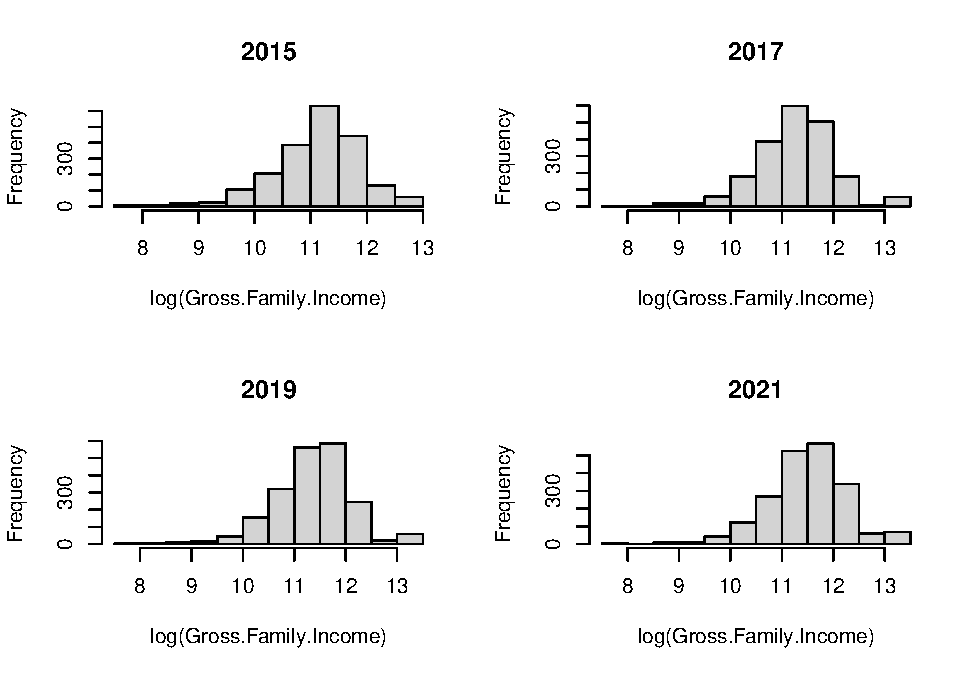
\includegraphics[keepaspectratio]{Vignette-for-panelTVP_files/figure-latex/unnamed-chunk-12-1.pdf}}

The boxplots suggest that the income distribution differs by time point
and, thus, some covariates may differ in their effects as well.

The marginal distribution of the response by time point is given by

\begin{Shaded}
\begin{Highlighting}[]
\NormalTok{Y \textless{}{-} sort(unique(Income$Year))}
\NormalTok{par(mfrow = c(2,2))}
\NormalTok{for(i in 1:4) hist(Income[Income$t == i,]$Gross.Family.Income\_log, main = Y[i],}
\NormalTok{                   xlab = "log(Gross.Family.Income)")}
\end{Highlighting}
\end{Shaded}

\pandocbounded{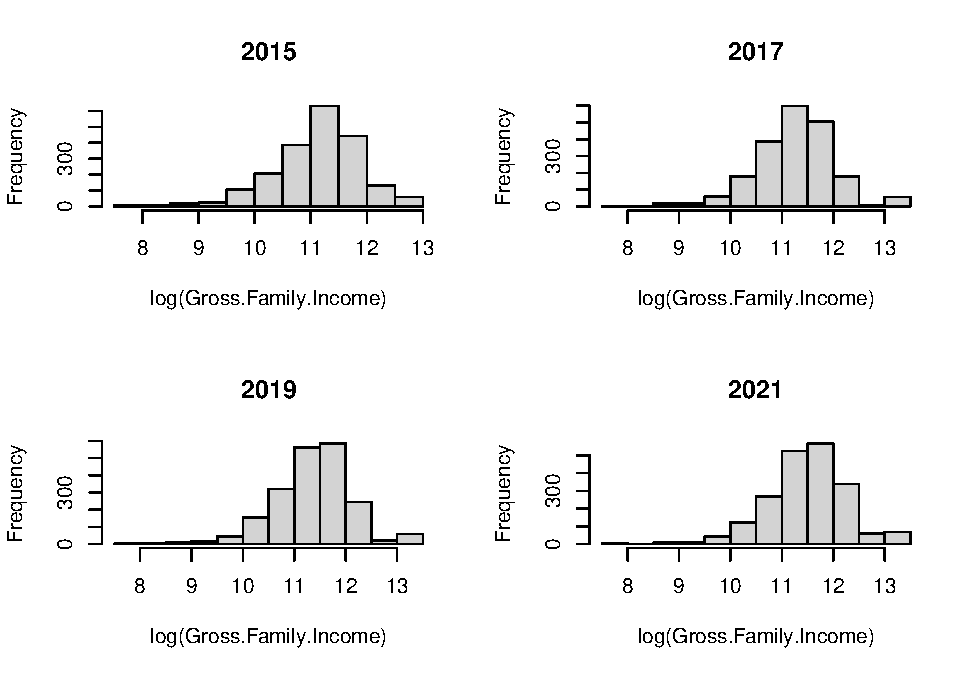
\includegraphics[keepaspectratio]{Vignette-for-panelTVP_files/figure-latex/unnamed-chunk-13-1.pdf}}

\begin{Shaded}
\begin{Highlighting}[]
\NormalTok{layout(1)}
\end{Highlighting}
\end{Shaded}

Despite the slightly left-skewed marginal distribution of the response,
we fit a Gaussian model with time-varying parameters by executing the
following code:

\begin{Shaded}
\begin{Highlighting}[]
\NormalTok{f.Gauss \textless{}{-} Gross.Family.Income\_log \textasciitilde{} Sex + Baseline.Age\_c + Ethnicity + Edu + Hours.Worked}
\NormalTok{Gauss.vignette \textless{}{-} panelTVP(formula = f.Gauss,}
\NormalTok{                           data = Income,}
\NormalTok{                           id = Income$id,}
\NormalTok{                           t = Income$t,}
\NormalTok{                           model = "Gaussian")}
\end{Highlighting}
\end{Shaded}

Information on the duration of the MCMC sampler can be accessed via

\begin{Shaded}
\begin{Highlighting}[]
\NormalTok{Gauss.vignette$runtime}
\end{Highlighting}
\end{Shaded}

\begin{verbatim}
## [1] "Total Runtime for Bayesian Normal Model: 182.35 seconds"
\end{verbatim}

The model comprises a lot of parameters, but the most important ones are
the time-varying regression effects and factor loadings. The S3
functions \texttt{summary()} and \texttt{plot()} can be used to show
those effects in a table and in a plot, respectively.

When summarizing the results in a table, the user can order the results
either by covariate or by time point, i.e.,

\begin{Shaded}
\begin{Highlighting}[]
\NormalTok{summary(Gauss.vignette)}
\end{Highlighting}
\end{Shaded}

\begin{verbatim}
## 
## ------------------------------------------------------------------------------
## Posterior Summary of the Bayesian Normal Model with Time-Varying Coefficients:
## ------------------------------------------------------------------------------
\end{verbatim}

\begin{verbatim}
## Warning in center_text(paste("Estimates for", nami[i])): At least one variable
## name is too long for fully displaying it.
\end{verbatim}

\begin{verbatim}
## ==================================================
##             Estimates for (Intercept)
## ==================================================
## 
##     Lower (HPD) Posterior Mean Upper (HPD)     SD
## t=1     10.1770        10.3579     10.5389 0.0919
## t=2     10.2783        10.4612     10.6299 0.0890
## t=3     10.4387        10.6017     10.8027 0.0896
## t=4     10.5488        10.7237     10.9099 0.0904
## 
## ==================================================
##              Estimates for Sexfemale
## ==================================================
## 
##     Lower (HPD) Posterior Mean Upper (HPD)     SD
## t=1     -0.1150        -0.0538      0.0082 0.0326
## t=2     -0.1394        -0.0778     -0.0233 0.0308
## t=3     -0.1548        -0.0971     -0.0341 0.0310
## t=4     -0.1682        -0.1047     -0.0468 0.0319
## 
## ==================================================
##            Estimates for Baseline.Age_c
## ==================================================
## 
##     Lower (HPD) Posterior Mean Upper (HPD)     SD
## t=1     -0.0033         0.0120      0.0321 0.0107
## t=2     -0.0044         0.0107      0.0305 0.0101
## t=3     -0.0051         0.0101      0.0297 0.0099
## t=4     -0.0076         0.0086      0.0294 0.0099
## 
## ==================================================
##          Estimates for EthnicityHispanic
## ==================================================
## 
##     Lower (HPD) Posterior Mean Upper (HPD)     SD
## t=1      0.1923         0.2753      0.3494 0.0408
## t=2      0.1968         0.2743      0.3528 0.0405
## t=3      0.1901         0.2729      0.3487 0.0406
## t=4      0.1913         0.2711      0.3521 0.0416
## 
## ==================================================
## Estimates for EthnicityMixed Race / Non-Black / No
## ==================================================
## 
##     Lower (HPD) Posterior Mean Upper (HPD)     SD
## t=1      0.3335         0.4026      0.4691 0.0348
## t=2      0.3481         0.4082      0.4777 0.0344
## t=3      0.3377         0.4029      0.4686 0.0346
## t=4      0.3471         0.4087      0.4802 0.0346
## 
## ==================================================
##        Estimates for Eduhigh school degree
## ==================================================
## 
##     Lower (HPD) Posterior Mean Upper (HPD)     SD
## t=1      0.0921         0.2419      0.3833 0.0751
## t=2      0.0894         0.2379      0.3655 0.0735
## t=3      0.0912         0.2313      0.3757 0.0745
## t=4      0.0780         0.2262      0.3757 0.0764
## 
## ==================================================
##          Estimates for Educollege degree
## ==================================================
## 
##     Lower (HPD) Posterior Mean Upper (HPD)     SD
## t=1      0.4449         0.5980      0.7433 0.0769
## t=2      0.4693         0.6148      0.7510 0.0744
## t=3      0.4776         0.6224      0.7620 0.0753
## t=4      0.4788         0.6220      0.7710 0.0762
## 
## ==================================================
## Estimates for Hours.Workedworked at least 30 hours
## ==================================================
## 
##     Lower (HPD) Posterior Mean Upper (HPD)     SD
## t=1      0.0369         0.1005      0.1721 0.0342
## t=2      0.0394         0.1074      0.1704 0.0330
## t=3      0.0343         0.0996      0.1731 0.0348
## t=4      0.0345         0.1089      0.1793 0.0359
## 
## ==================================================
##            Estimates for Factor Loading
## ==================================================
## 
##     Lower (HPD) Posterior Mean Upper (HPD)     SD
## t=1      0.5218         0.5430      0.5658 0.0112
## t=2      0.5232         0.5464      0.5701 0.0120
## t=3      0.5147         0.5369      0.5591 0.0117
## t=4      0.5208         0.5432      0.5672 0.0119
\end{verbatim}

\begin{Shaded}
\begin{Highlighting}[]
\NormalTok{summary(Gauss.vignette, by = "timepoint")}
\end{Highlighting}
\end{Shaded}

\begin{verbatim}
## 
## ------------------------------------------------------------------------------
## Posterior Summary of the Bayesian Normal Model with Time-Varying Coefficients:
## ------------------------------------------------------------------------------
## ==================================================
##             Estimates for Timepoint 1
## ==================================================
## 
##                                                Lower (HPD) Posterior Mean
## (Intercept)                                        10.1770        10.3579
## Sexfemale                                          -0.1150        -0.0538
## Baseline.Age_c                                     -0.0033         0.0120
## EthnicityHispanic                                   0.1923         0.2753
## EthnicityMixed Race / Non-Black / Non-Hispanic      0.3335         0.4026
## Eduhigh school degree                               0.0921         0.2419
## Educollege degree                                   0.4449         0.5980
## Hours.Workedworked at least 30 hours                0.0369         0.1005
## Factor Loading                                      0.5218         0.5430
##                                                Upper (HPD)     SD
## (Intercept)                                        10.5389 0.0919
## Sexfemale                                           0.0082 0.0326
## Baseline.Age_c                                      0.0321 0.0107
## EthnicityHispanic                                   0.3494 0.0408
## EthnicityMixed Race / Non-Black / Non-Hispanic      0.4691 0.0348
## Eduhigh school degree                               0.3833 0.0751
## Educollege degree                                   0.7433 0.0769
## Hours.Workedworked at least 30 hours                0.1721 0.0342
## Factor Loading                                      0.5658 0.0112
## 
## ==================================================
##             Estimates for Timepoint 2
## ==================================================
## 
##                                                Lower (HPD) Posterior Mean
## (Intercept)                                        10.2783        10.4612
## Sexfemale                                          -0.1394        -0.0778
## Baseline.Age_c                                     -0.0044         0.0107
## EthnicityHispanic                                   0.1968         0.2743
## EthnicityMixed Race / Non-Black / Non-Hispanic      0.3481         0.4082
## Eduhigh school degree                               0.0894         0.2379
## Educollege degree                                   0.4693         0.6148
## Hours.Workedworked at least 30 hours                0.0394         0.1074
## Factor Loading                                      0.5232         0.5464
##                                                Upper (HPD)     SD
## (Intercept)                                        10.6299 0.0890
## Sexfemale                                          -0.0233 0.0308
## Baseline.Age_c                                      0.0305 0.0101
## EthnicityHispanic                                   0.3528 0.0405
## EthnicityMixed Race / Non-Black / Non-Hispanic      0.4777 0.0344
## Eduhigh school degree                               0.3655 0.0735
## Educollege degree                                   0.7510 0.0744
## Hours.Workedworked at least 30 hours                0.1704 0.0330
## Factor Loading                                      0.5701 0.0120
## 
## ==================================================
##             Estimates for Timepoint 3
## ==================================================
## 
##                                                Lower (HPD) Posterior Mean
## (Intercept)                                        10.4387        10.6017
## Sexfemale                                          -0.1548        -0.0971
## Baseline.Age_c                                     -0.0051         0.0101
## EthnicityHispanic                                   0.1901         0.2729
## EthnicityMixed Race / Non-Black / Non-Hispanic      0.3377         0.4029
## Eduhigh school degree                               0.0912         0.2313
## Educollege degree                                   0.4776         0.6224
## Hours.Workedworked at least 30 hours                0.0343         0.0996
## Factor Loading                                      0.5147         0.5369
##                                                Upper (HPD)     SD
## (Intercept)                                        10.8027 0.0896
## Sexfemale                                          -0.0341 0.0310
## Baseline.Age_c                                      0.0297 0.0099
## EthnicityHispanic                                   0.3487 0.0406
## EthnicityMixed Race / Non-Black / Non-Hispanic      0.4686 0.0346
## Eduhigh school degree                               0.3757 0.0745
## Educollege degree                                   0.7620 0.0753
## Hours.Workedworked at least 30 hours                0.1731 0.0348
## Factor Loading                                      0.5591 0.0117
## 
## ==================================================
##             Estimates for Timepoint 4
## ==================================================
## 
##                                                Lower (HPD) Posterior Mean
## (Intercept)                                        10.5488        10.7237
## Sexfemale                                          -0.1682        -0.1047
## Baseline.Age_c                                     -0.0076         0.0086
## EthnicityHispanic                                   0.1913         0.2711
## EthnicityMixed Race / Non-Black / Non-Hispanic      0.3471         0.4087
## Eduhigh school degree                               0.0780         0.2262
## Educollege degree                                   0.4788         0.6220
## Hours.Workedworked at least 30 hours                0.0345         0.1089
## Factor Loading                                      0.5208         0.5432
##                                                Upper (HPD)     SD
## (Intercept)                                        10.9099 0.0904
## Sexfemale                                          -0.0468 0.0319
## Baseline.Age_c                                      0.0294 0.0099
## EthnicityHispanic                                   0.3521 0.0416
## EthnicityMixed Race / Non-Black / Non-Hispanic      0.4802 0.0346
## Eduhigh school degree                               0.3757 0.0764
## Educollege degree                                   0.7710 0.0762
## Hours.Workedworked at least 30 hours                0.1793 0.0359
## Factor Loading                                      0.5672 0.0119
\end{verbatim}

Effect plots can be easily obtained as

\begin{Shaded}
\begin{Highlighting}[]
\NormalTok{plot(Gauss.vignette, nplots = 2)}
\end{Highlighting}
\end{Shaded}

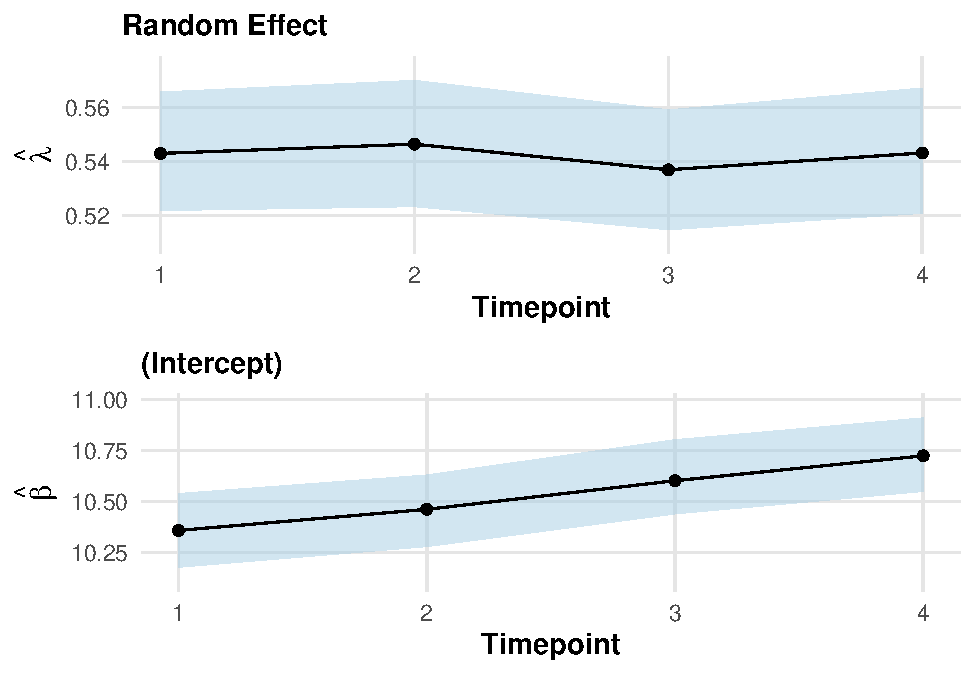
\includegraphics[width=0.7\linewidth]{Vignette-for-panelTVP_files/figure-latex/myplot-1}

\begin{verbatim}
## The plots are out there, hit [Return] to see ...
\end{verbatim}

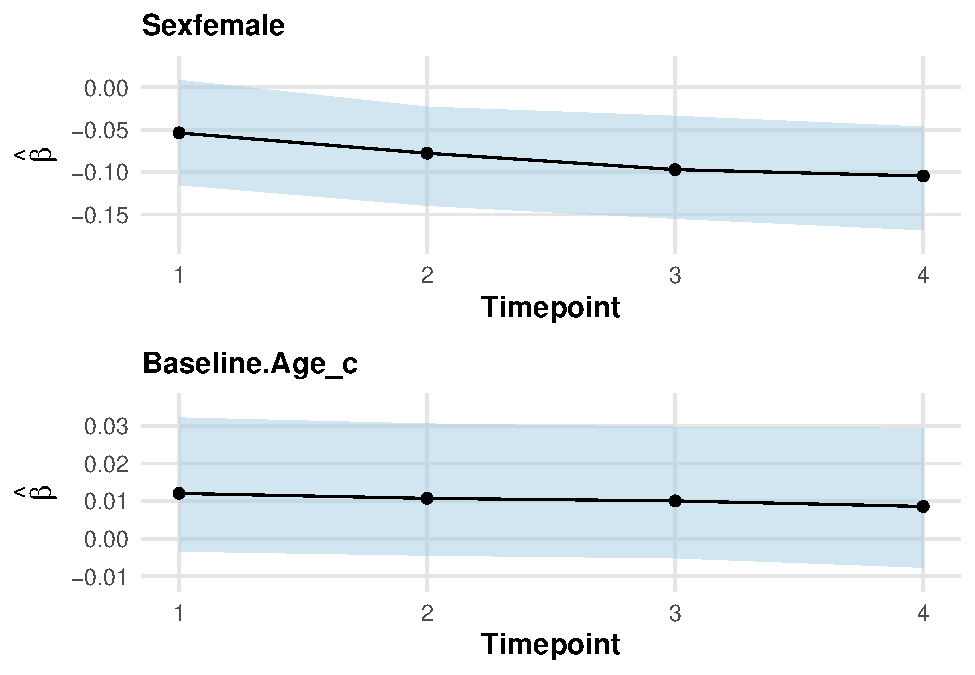
\includegraphics[width=0.7\linewidth]{Vignette-for-panelTVP_files/figure-latex/myplot-2}

\begin{verbatim}
## The plots are out there, hit [Return] to see ...
\end{verbatim}

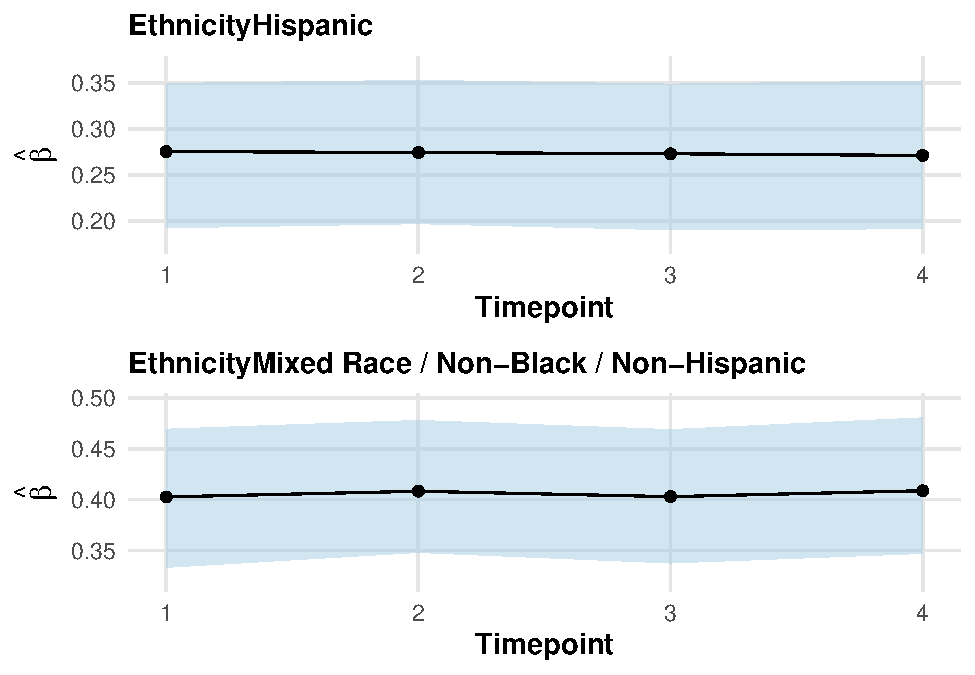
\includegraphics[width=0.7\linewidth]{Vignette-for-panelTVP_files/figure-latex/myplot-3}

\begin{verbatim}
## The plots are out there, hit [Return] to see ...
\end{verbatim}

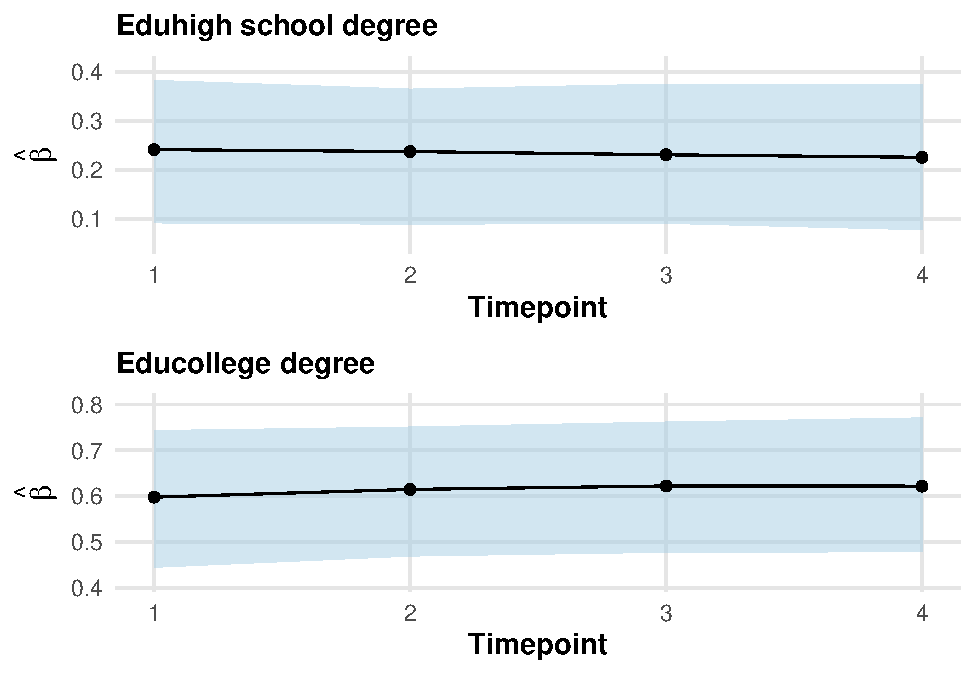
\includegraphics[width=0.7\linewidth]{Vignette-for-panelTVP_files/figure-latex/myplot-4}

\begin{verbatim}
## The plots are out there, hit [Return] to see ...
\end{verbatim}

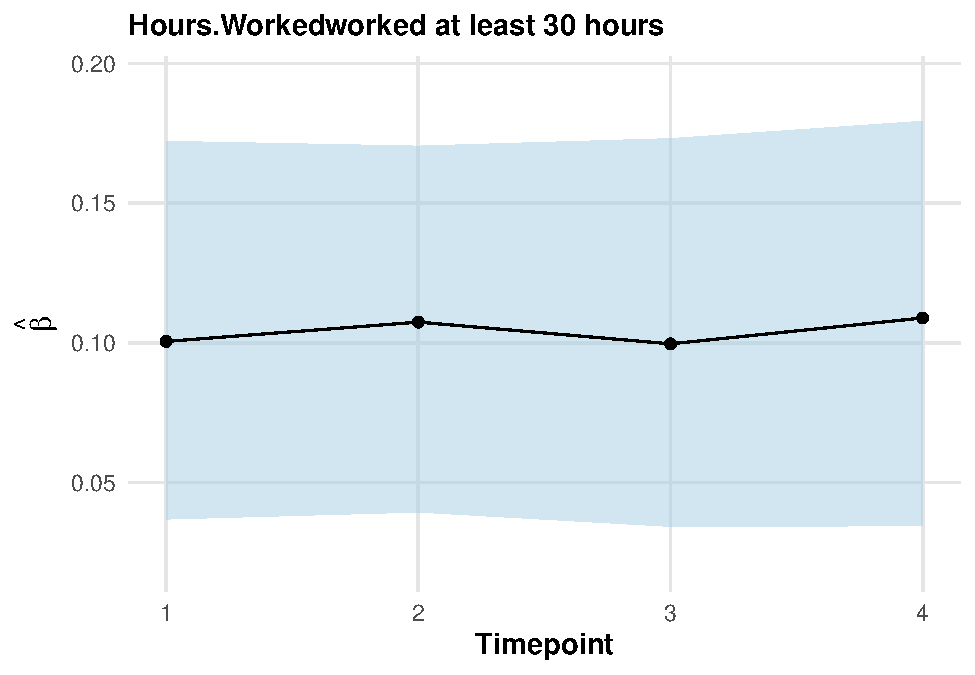
\includegraphics[width=0.7\linewidth]{Vignette-for-panelTVP_files/figure-latex/myplot-5}

The first effect plot is always the random effect or the factor loading,
which is followed by the global intercept. Afterwards, the time-varying
effects of covariates are given. Based on the results we observe an
increase in the overall income level over time and a decrease for the
women. Hence, the interviewed women have ceteris paribus a lower gross
family income than men and this effect is more pronounced as they get
older. The other effect estimates are shrunken to time-invariance. We
see that people with a high school or college degree earn on average
more money (or at least have a higher family income) than people with no
completed degree. Furthermore, working at least 30 hours yields an
increase in the gross family income compared to people who work less
than 30 hours.

Aside from the inspection of the time-varying parameters, Bayesian
inference with MCMC requires proper evaluation of the generated Markov
Chains. The remaining MCMC draws after burn-in and thinning for all
parameters are stored in the matrix \texttt{mcmc}, i.e.,

\begin{Shaded}
\begin{Highlighting}[]
\NormalTok{head(Gauss.vignette$mcmc, 4)}
\end{Highlighting}
\end{Shaded}

\begin{verbatim}
##      beta_t11 beta_t12 beta_t13 beta_t14    beta_t21    beta_t22   beta_t23
## [1,] 10.44387 10.54999 10.68535 10.75595 -0.11399866 -0.12826341 -0.1332617
## [2,] 10.36887 10.49241 10.66686 10.79378 -0.02807614 -0.07490815 -0.1002995
## [3,] 10.43375 10.52945 10.67197 10.79683 -0.01333708 -0.07377731 -0.1235973
## [4,] 10.36396 10.47429 10.58853 10.70264 -0.06882912 -0.11018192 -0.1505653
##         beta_t24      beta_t31      beta_t32      beta_t33      beta_t34
## [1,] -0.15070571  3.702441e-03  0.0037157278  0.0038962246  0.0023979584
## [2,] -0.09927611  3.768037e-04  0.0006411826 -0.0002872084 -0.0001843646
## [3,] -0.10039401 -4.095493e-05 -0.0001094372 -0.0001362720 -0.0002314573
## [4,] -0.13846180  2.076244e-02  0.0107683800  0.0100131834  0.0022898896
##       beta_t41  beta_t42  beta_t43  beta_t44  beta_t51  beta_t52  beta_t53
## [1,] 0.1919325 0.1919116 0.1918210 0.1920599 0.3706134 0.4097664 0.3443580
## [2,] 0.1868633 0.1875196 0.1874116 0.1862384 0.3765959 0.3757303 0.3747769
## [3,] 0.2265296 0.2264692 0.2270813 0.2264614 0.4408758 0.4405047 0.4403487
## [4,] 0.3051175 0.3041564 0.3047913 0.3050399 0.4242387 0.4773669 0.4232808
##       beta_t54  beta_t61  beta_t62  beta_t63  beta_t64  beta_t71  beta_t72
## [1,] 0.3955467 0.2243026 0.2223148 0.2226232 0.2458123 0.5692582 0.5955511
## [2,] 0.3757758 0.2667827 0.2425325 0.2119134 0.1745347 0.6058749 0.6058278
## [3,] 0.4406143 0.1917788 0.1917759 0.1917791 0.1917729 0.4869194 0.5516268
## [4,] 0.4446442 0.2301241 0.2301311 0.2301256 0.2301233 0.5843568 0.5902506
##       beta_t73  beta_t74   beta_t81  beta_t82   beta_t83   beta_t84    beta1
## [1,] 0.6142144 0.6411122 0.10302578 0.1055438 0.10702309 0.10845499 10.51355
## [2,] 0.6058872 0.6061404 0.12043767 0.1267505 0.12518459 0.13211203 10.49056
## [3,] 0.5633139 0.5696016 0.10480391 0.1143182 0.08238619 0.08364508 10.36190
## [4,] 0.5838170 0.5735417 0.07953443 0.0848327 0.14585243 0.15456917 10.59974
##             beta2         beta3     beta4     beta5     beta6     beta7
## [1,] -0.037905304  7.540648e-03 0.1919981 0.2145166 0.2201216 0.5741728
## [2,] -0.004879238  2.063433e-07 0.1864386 0.3781858 0.2670730 0.6058916
## [3,] -0.009461096  1.607629e-07 0.2262566 0.4410600 0.1917904 0.3527311
## [4,] -0.052205094 -1.959871e-07 0.3055418 0.4083764 0.2301097 0.5820129
##           beta8     theta1      theta2       theta3        theta4       theta5
## [1,] 0.09958768 -0.1244162  0.05620747 0.0020570045 -0.0001079763 0.1029707474
## [2,] 0.13277618 -0.1279928  0.01812659 0.0005113931 -0.0017106338 0.0007763536
## [3,] 0.14199795 -0.1070822  0.03033023 0.0001314508  0.0005025183 0.0002887696
## [4,] 0.11492109  0.1158389 -0.04157812 0.0112413837 -0.0009651928 0.0619698782
##             theta6        theta7       theta8     tau21        tau22
## [1,] -7.943579e-03 -0.0365450695 -0.001998671  60.71629 0.0053509274
## [2,] -4.010307e-02  0.0002463352 -0.012090209  61.58600 0.0115708661
## [3,] -5.279756e-06 -0.1199411879  0.028257506 162.02628 0.0001783864
## [4,]  1.060278e-05 -0.0139054569 -0.044650712  58.78335 0.0116680637
##             tau23      tau24      tau25       tau26      tau27       tau28
## [1,] 7.020765e-05 0.01193802 65.4477443 187.7544372 0.16867667  0.07579487
## [2,] 3.795668e-13 0.05206231  0.1475576   0.2763538 1.50798234 16.27691262
## [3,] 3.146930e-14 8.46000716 16.2338844   0.1963824 0.03801637  0.15360257
## [4,] 5.258971e-14 3.58657134 13.2951325   0.1410246 0.46093041  1.12431768
##             xi21        xi22         xi23         xi24         xi25
## [1,] 0.171369511 0.007066971 5.773325e-04 4.294428e-08 2.054407e-03
## [2,] 0.302247597 0.002154247 1.131716e-07 3.568133e-06 6.115310e-07
## [3,] 0.007075938 0.039362529 1.691021e-06 3.387866e-05 3.890994e-04
## [4,] 0.007400079 0.012309663 1.377170e-03 1.664418e-05 2.102253e-03
##              xi26         xi27         xi28      a.tau kappa.tau      a.xi
## [1,] 3.102158e-05 4.801811e-04 9.541107e-05 0.14985253 0.1297529 0.1329226
## [2,] 2.724440e-03 5.511761e-08 1.528679e-04 0.08159118 0.7632204 0.1215459
## [3,] 8.516701e-10 5.384080e-02 6.443829e-02 0.11601315 0.1173748 0.1349858
## [4,] 5.217748e-06 8.746377e-04 4.541086e-04 0.08097238 0.1109783 0.1495742
##       kappa.xi    sigma2 lambda_t1 lambda_t2 lambda_t3 lambda_t4    lambda
## [1,]  88.92907 0.1788861 0.5389640 0.5406923 0.5281776 0.5472028 0.5333181
## [2,]  54.04817 0.1811933 0.5449713 0.5395289 0.5340582 0.5444099 0.5409153
## [3,]  15.08552 0.1840817 0.5389138 0.5327645 0.5355356 0.5330704 0.5357220
## [4,] 449.32039 0.1846950 0.5345261 0.5465252 0.5414073 0.5362844 0.5375839
##               psi       phi2       zeta2 a.phi    kappa.phi a.zeta   kappa.zeta
## [1,] -0.022275078 61.2992209 0.039290394     1  0.048936634      1   32.2354402
## [2,] -0.021067576  0.4959154 0.001097921     1  0.007379546      1 1296.1812925
## [3,]  0.007318261  0.1190598 0.009182661     1 16.354238412      1  106.1703867
## [4,]  0.005572515  9.0650754 1.031545035     1  0.283040547      1    0.5351148
\end{verbatim}

The first columns are the sampled draws of the time-varying regression
effects and, thus, the most interesting parameters. The first covariate
is usually the global intercept. When using a random walk shrinkage
prior, you also get the ``fixed'' effects or starting values of the
random walks, which are in this case
\texttt{beta1}\(,\dots,\)\texttt{beta8}, as well as the scale parameters
of the random walks, which are in this case
\texttt{theta1}\(,\dots,\)\texttt{theta8}. The next parameters are the
hyperparameters of the shrinkage priors, which are in this case
\texttt{tau21}\(,\dots,\)\texttt{tau28},
\texttt{xi21}\(,\dots,\)\texttt{xi28}, \texttt{a.tau}, \texttt{a.xi},
\texttt{kappa.tau}, \texttt{kappa.xi}. As we have fitted a Normal
regression model, the homoscedastic error variance \texttt{sigma2} is
also contained in the matrix. For a count regression model, the
dispersion parameter \texttt{r} of the Negative Binomial distribution
will be included instead. The remaining parameters relate to the factor
loadings, but are otherwise similar to the corresponding parameters for
the regression part of the model.

The chains can then be analyzed to assess convergence to the stationary
distributions. For visual diagnostics, traceplots and plots of the ACFs
are useful, e.g.,

\begin{Shaded}
\begin{Highlighting}[]
\NormalTok{par(mfrow = c(2,2))}
\NormalTok{plot(Gauss.vignette$mcmc[,"beta\_t11"], type = "l", }
\NormalTok{     main = "Trace of beta\_t11 (Intercept at t = 1)", xlab = "", ylab = "")}
\NormalTok{acf(Gauss.vignette$mcmc[,"beta\_t11"],}
\NormalTok{    main = "ACF of beta\_t11 (Intercept at t = 1)")}
\NormalTok{plot(Gauss.vignette$mcmc[,"lambda\_t1"], type = "l", }
\NormalTok{     main = "Trace of lambda\_t1 (Loading at t = 1)", xlab = "", ylab = "")}
\NormalTok{acf(Gauss.vignette$mcmc[,"lambda\_t1"],}
\NormalTok{    main = "ACF of lambda\_t1 (Loading at t = 1)")}
\end{Highlighting}
\end{Shaded}

\pandocbounded{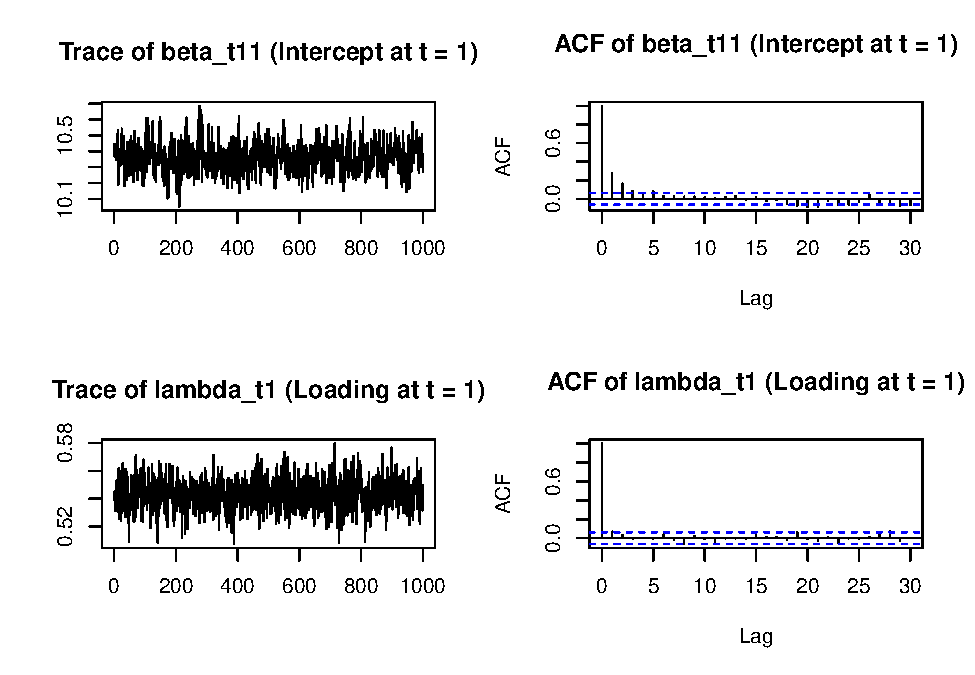
\includegraphics[keepaspectratio]{Vignette-for-panelTVP_files/figure-latex/unnamed-chunk-20-1.pdf}}

\begin{Shaded}
\begin{Highlighting}[]
\NormalTok{layout(1)}
\end{Highlighting}
\end{Shaded}

A quantity for summarizing the information in a correlated sample in a
single number is the effective sample size (ESS), which is defined as

\begin{equation*}
 \text{ESS} = \frac{M}{1+2\sum_{s=1}^\infty \rho_s}, 
\end{equation*} where \(M\) is the length of the chain (after burn-in
and thinning) and \(\rho_s\) is the autocorrelation of the chain at lag
\(s\). The ESS can be interpreted as the number of independent draws
that is equivalent to \(M\) MCMC draws. This parameter-specific quantity
can be computed as

\begin{Shaded}
\begin{Highlighting}[]
\NormalTok{LaplacesDemon::ESS(Gauss.vignette$mcmc[,"lambda\_t1"])}
\end{Highlighting}
\end{Shaded}

\begin{verbatim}
## [1] 872.7779
\end{verbatim}

As the length of the Markov Chain is \(M = 1000\), we conclude that
enough information was used for estimating the factor loading at the
first time point.

The variables are coded in the order of their inclusion in the
\texttt{formula} argument. For \texttt{summary()} and \texttt{plot()}
the actual variable labels are used. However, this is not the case for,
e.g., the \texttt{mcmc} object. For this, the object
\texttt{variable.codes} was created, which maps the variable labels to
their codes, i.e.,

\begin{Shaded}
\begin{Highlighting}[]
\NormalTok{Gauss.vignette$variable.codes}
\end{Highlighting}
\end{Shaded}

\begin{verbatim}
##      variable                                         effect 
## [1,] "(Intercept)"                                    "beta1"
## [2,] "Sexfemale"                                      "beta2"
## [3,] "Baseline.Age_c"                                 "beta3"
## [4,] "EthnicityHispanic"                              "beta4"
## [5,] "EthnicityMixed Race / Non-Black / Non-Hispanic" "beta5"
## [6,] "Eduhigh school degree"                          "beta6"
## [7,] "Educollege degree"                              "beta7"
## [8,] "Hours.Workedworked at least 30 hours"           "beta8"
\end{verbatim}

Finally, it should be mentioned how samples from the posterior
predictive distribution can be obtained for the models fitted with
\texttt{panelTVP()}. The object \texttt{posterior.predictive} contains
\(M\) draws from the posterior predictive distribution of the fitted
values, i.e., the values of the response variable that were used for
training the model. The object is a matrix where each row corresponds to
an observation in the training data and each column to a draw of the
Markov Chain (after burn-in and thinning).

\begin{Shaded}
\begin{Highlighting}[]
\NormalTok{dim(Gauss.vignette$posterior.predictive)}
\end{Highlighting}
\end{Shaded}

\begin{verbatim}
## [1] 8060 1000
\end{verbatim}

The posterior predictive distribution of the training data can be used
for posterior predictive checks (PPC). Functions to perform PPC are,
e.g., available in the \texttt{bayesplot} package. One way of assessing
the fit of a Bayesian model is to superimpose the density of the
original data with the \(M\) densities of the posterior predictive
distribution.

\begin{Shaded}
\begin{Highlighting}[]
\NormalTok{bayesplot::ppc\_dens\_overlay(y = Income$Gross.Family.Income\_log,}
\NormalTok{                            yrep = t(Gauss.vignette$posterior.predictive))}
\end{Highlighting}
\end{Shaded}

\pandocbounded{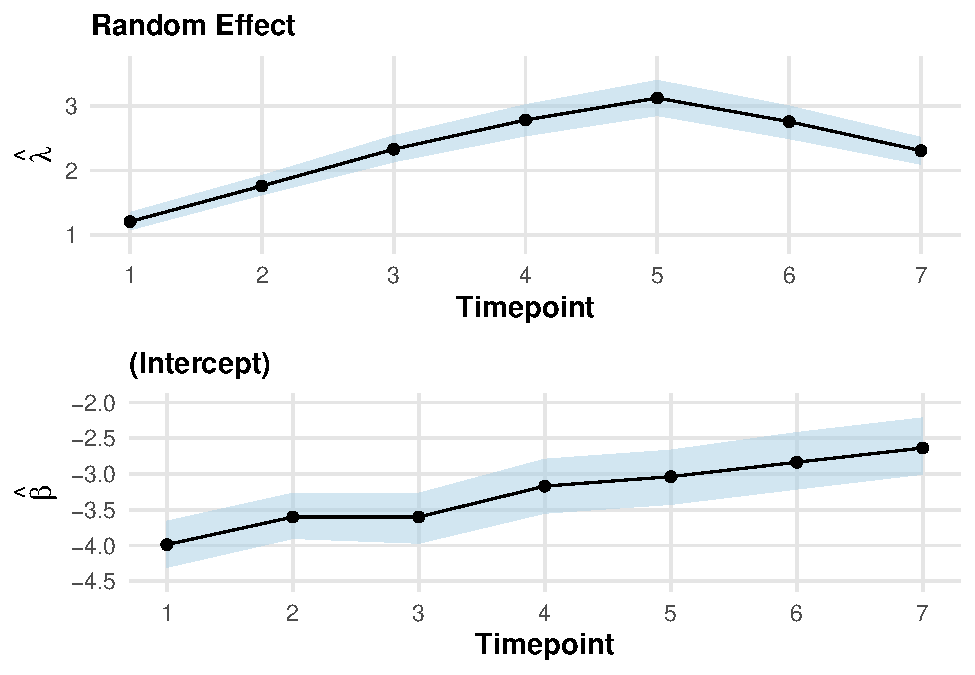
\includegraphics[keepaspectratio]{Vignette-for-panelTVP_files/figure-latex/unnamed-chunk-24-1.pdf}}

Although the predicted densities are close to the density of the
training data, we see that the pronounced peak at a log-income value of
around \(11.5\) is not fully captured. Moreover, information on the
small peak located at the right tail of the distribution is not
contained in the posterior predictive distributions.

It is also possible to make predictions for new data using the S3
function \texttt{predict()}. This function has the following structure:

\begin{Shaded}
\begin{Highlighting}[]
\NormalTok{predict(object, X.new, timepoint, coverage = 0.95,}
\NormalTok{        pop.pred = FALSE, n.replicates = 100, ...)}
\end{Highlighting}
\end{Shaded}

The argument \texttt{object} is an object that is returned by
\texttt{panelTVP()}. The argument \texttt{X.new} is a \texttt{matrix} or
a \texttt{data.frame} object, which contains the new data. Predictions
are made for a specific time point that is specified in the argument
\texttt{timepoint}. In addition to point predictions, Bayesian HPD
prediction intervals are obtained as well with coverage probability that
can be defined by using the argument \texttt{coverage}. The argument
\texttt{pop.pred} is a Boolean and indicates whether the posterior
predictive distribution of new data should be based on the population
level or if random effects / factors should be included as well. If
\texttt{pop.pred = FALSE}, then the subject-specific factors are
integrated out as for new data subject-specific information is not
available. For marginalization, \texttt{n.replicates} samples are drawn,
where the latent factors are simulated from the prior. Therefore, the
accuracy of marginalization increases as \texttt{n.replicates} increases
- at the cost of increased computational complexity.

In the following, the prediction task is briefly demonstrated. Suppose
we want to make predictions for a specific time point for two new
subjects for our \texttt{Income} data. For this, we first set up the new
design matrix and then run the \texttt{predict()} function:

\begin{Shaded}
\begin{Highlighting}[]
\NormalTok{names.orig \textless{}{-} colnames(Gauss.vignette$data$X)}

\NormalTok{X.new \textless{}{-} data.frame(Intercept = c(1,1),}
\NormalTok{                    Sex = c(0,1),}
\NormalTok{                    Baseline.Age\_c = c(12,16),}
\NormalTok{                    EthnicityHispanic = c(1,0),}
\NormalTok{                    EthnicityMixed = c(0,0),}
\NormalTok{                    highschool = c(1,0),}
\NormalTok{                    college = c(0,1),}
\NormalTok{                    Hours.Worked = c(0,1))}
\NormalTok{colnames(X.new) \textless{}{-} names.orig}

\NormalTok{pp \textless{}{-} predict(object = Gauss.vignette,}
\NormalTok{              X.new = X.new,}
\NormalTok{              timepoint = 4)}
\end{Highlighting}
\end{Shaded}

The object \texttt{pp} is a list consisting of two matrices. The matrix
\texttt{predictive.summary} contains summary statistics derived from the
predictive distribution, i.e.,

\begin{Shaded}
\begin{Highlighting}[]
\NormalTok{pp$predictive.summary}
\end{Highlighting}
\end{Shaded}

\begin{verbatim}
##         LO     mean       UP
## 1 11.09476 11.32202 11.56590
## 2 11.24418 11.48579 11.78983
\end{verbatim}

The matrix \texttt{predictive.distribution} contains the posterior
predictive distribution and is of dimension \(N_{new} \times M\), where
\(N_{new}\) is the number of new data points.

\begin{Shaded}
\begin{Highlighting}[]
\NormalTok{par(mfrow = c(2,1))}

\NormalTok{hist(pp$predictive.distribution[1,], }
\NormalTok{     main = "Predictive Distribution of First New Subject",}
\NormalTok{     xlab = "log(Gross.Family.Income)",}
\NormalTok{     xlim = c(10.8,12.2),}
\NormalTok{     breaks = 25)}

\NormalTok{hist(pp$predictive.distribution[2,], }
\NormalTok{     main = "Predictive Distribution of Second New Subject",}
\NormalTok{     xlab = "log(Gross.Family.Income)",}
\NormalTok{     xlim = c(10.8,12.2),}
\NormalTok{     breaks = 25)}
\end{Highlighting}
\end{Shaded}

\pandocbounded{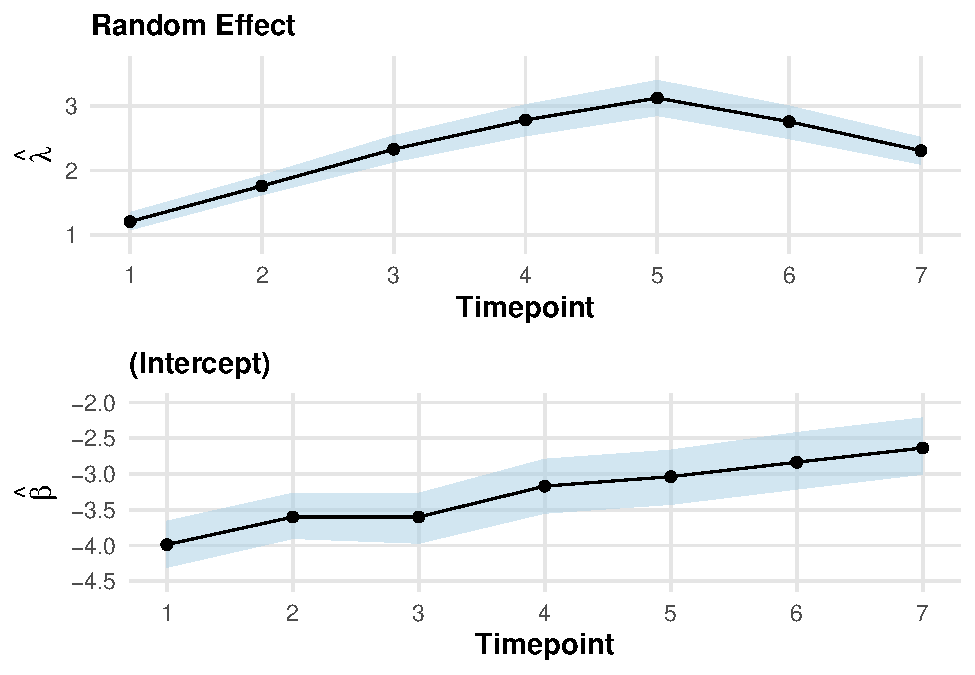
\includegraphics[keepaspectratio]{Vignette-for-panelTVP_files/figure-latex/unnamed-chunk-28-1.pdf}}

\begin{Shaded}
\begin{Highlighting}[]
\NormalTok{layout(1)}
\end{Highlighting}
\end{Shaded}

\section{Analyzing binary response
data}\label{analyzing-binary-response-data}

In this section we focus on the analysis of binary outcomes using the
Logit model. A corresponding Probit regression model can easily be set
up by changing the \texttt{model} argument accordingly and, thus, will
not be discussed here.

For demonstration, we will use the \texttt{Marijuana} dataset that is
contained in the \texttt{panelTVP} package. This dataset is a
pre-processed subset of the
\textit{National Longitudinal Survey of Youth 1997} and contains data of
the first seven waves of this study. The response variable is
\texttt{Used.Mari.Since.DLI} and indicates if the person has consumed
Marijuana since the last interview date. A one means that the person has
consumed the drug. For the first wave the question was, if the person
has ever consumed Marijuana in his/her life. The goal is to explain the
probability of Marijuana consumption as a function of covariates and to
assess whether effects of covariates are subject to temporal change.

To get an overview of the data, the first 10 rows are given in the
following:

\begin{Shaded}
\begin{Highlighting}[]
\NormalTok{head(Marijuana, 10)}
\end{Highlighting}
\end{Shaded}

\begin{verbatim}
##     Bullied.Before.12    Sex                             Ethnicity Year Age
## 1                  no female Mixed Race / Non-Black / Non-Hispanic 1997  15
## 10                yes   male                              Hispanic 1997  14
## 22                 no female                              Hispanic 1997  15
## 35                 no   male                              Hispanic 1997  15
## 52                 no female Mixed Race / Non-Black / Non-Hispanic 1997  16
## 57                 no   male Mixed Race / Non-Black / Non-Hispanic 1997  15
## 64                 no   male Mixed Race / Non-Black / Non-Hispanic 1997  14
## 72                 no female                              Hispanic 1997  15
## 84                yes   male                              Hispanic 1997  15
## 103                no female                              Hispanic 1997  15
##     Residence t id Baseline.Age_c Used.Mari.Since.DLI
## 1       Urban 1  1              3                   0
## 10      Urban 1  2              2                   0
## 22      Urban 1  4              3                   0
## 35      Urban 1  5              3                   1
## 52      Urban 1  8              4                   0
## 57      Urban 1  9              3                   0
## 64      Urban 1 10              2                   0
## 72      Urban 1 11              3                   0
## 84      Urban 1 12              3                   0
## 103     Urban 1 15              3                   0
\end{verbatim}

The variable \texttt{Bullied.Before.12} indicates whether the person was
a victim of bullying before the age of 12. The variable
\texttt{Residence} gives information on the location where the person
lives in and is either \texttt{Urban} or \texttt{Rural}. Finally, the
variable \texttt{Baseline.Age\_c} is a centered version of the person's
baseline age at study begin.

A Bayesian Logit model with time-varying parameters and shrinkage priors
on the effects can be estimated as follows:

\begin{Shaded}
\begin{Highlighting}[]
\NormalTok{f.logit \textless{}{-} Used.Mari.Since.DLI \textasciitilde{} Sex + Baseline.Age\_c + Residence + Bullied.Before.12 + Ethnicity}
\NormalTok{logit.vignette \textless{}{-} panelTVP(formula = f.logit,}
\NormalTok{                           data = Marijuana,}
\NormalTok{                           id = Marijuana$id,}
\NormalTok{                           t = Marijuana$t,}
\NormalTok{                           model = "Logit")}
\end{Highlighting}
\end{Shaded}

The total runtime of the sampler was considerably longer than for the
Gaussian model. This is due to the fact that the Logit model requires
sampling of Pólya-Gamma weights in each step of the sampler.

\begin{Shaded}
\begin{Highlighting}[]
\NormalTok{logit.vignette$runtime}
\end{Highlighting}
\end{Shaded}

\begin{verbatim}
## [1] "Total Runtime for Bayesian Logit Model: 1092.35 seconds"
\end{verbatim}

The estimated effects can again be summarized in a table

\begin{Shaded}
\begin{Highlighting}[]
\NormalTok{summary(logit.vignette)}
\end{Highlighting}
\end{Shaded}

\begin{verbatim}
## ------------------------------------------------------------------------------
## Posterior Summary of the Bayesian Logit Model with Time-Varying Coefficients:
## -----------------------------------------------------------------------------
\end{verbatim}

\begin{verbatim}
## Warning in center_text(paste("Estimates for", nami[i])): At least one variable
## name is too long for fully displaying it.
\end{verbatim}

\begin{verbatim}
## ==================================================
##             Estimates for (Intercept)
## ==================================================
## 
##     Lower (HPD) Posterior Mean Upper (HPD)     SD
## t=1     -4.3070        -3.9889     -3.6606 0.1754
## t=2     -3.9034        -3.6023     -3.2692 0.1588
## t=3     -3.9702        -3.6012     -3.2705 0.1781
## t=4     -3.5495        -3.1704     -2.7928 0.1925
## t=5     -3.4261        -3.0374     -2.6662 0.1973
## t=6     -3.2125        -2.8364     -2.4198 0.2002
## t=7     -3.0040        -2.6366     -2.2144 0.2011
## 
## ==================================================
##              Estimates for Sexfemale
## ==================================================
## 
##     Lower (HPD) Posterior Mean Upper (HPD)     SD
## t=1     -0.3470        -0.1531     -0.0108 0.0856
## t=2     -0.3680        -0.1861     -0.0114 0.0889
## t=3     -0.4666        -0.2656     -0.0822 0.0969
## t=4     -0.6299        -0.4140     -0.1741 0.1181
## t=5     -0.6300        -0.4102     -0.1639 0.1185
## t=6     -0.8790        -0.6215     -0.3532 0.1358
## t=7     -0.6910        -0.4846     -0.2689 0.1122
## 
## ==================================================
##            Estimates for Baseline.Age_c
## ==================================================
## 
##     Lower (HPD) Posterior Mean Upper (HPD)     SD
## t=1      0.5691         0.6418      0.7138 0.0373
## t=2      0.2921         0.3676      0.4352 0.0366
## t=3      0.2114         0.2905      0.3697 0.0401
## t=4      0.0229         0.1134      0.1946 0.0446
## t=5     -0.1201        -0.0336      0.0598 0.0473
## t=6     -0.1527        -0.0597      0.0287 0.0465
## t=7     -0.2155        -0.1367     -0.0531 0.0418
## 
## ==================================================
##            Estimates for ResidenceUrban
## ==================================================
## 
##     Lower (HPD) Posterior Mean Upper (HPD)     SD
## t=1      0.0548         0.2184      0.4127 0.0958
## t=2      0.0924         0.2503      0.4436 0.0874
## t=3      0.0521         0.2380      0.4245 0.0976
## t=4      0.1414         0.3405      0.5276 0.0988
## t=5      0.1897         0.3898      0.5882 0.1035
## t=6      0.2713         0.5116      0.7420 0.1228
## t=7      0.2836         0.5654      0.8177 0.1363
## 
## ==================================================
##         Estimates for Bullied.Before.12yes
## ==================================================
## 
##     Lower (HPD) Posterior Mean Upper (HPD)     SD
## t=1      0.3574         0.5458      0.7252 0.0963
## t=2      0.3636         0.5426      0.7222 0.0948
## t=3      0.3535         0.5418      0.7309 0.0980
## t=4      0.3255         0.5312      0.7156 0.1011
## t=5      0.3244         0.5251      0.7281 0.1033
## t=6      0.3156         0.5179      0.7418 0.1083
## t=7      0.3290         0.5255      0.7404 0.1046
## 
## ==================================================
##          Estimates for EthnicityHispanic
## ==================================================
## 
##     Lower (HPD) Posterior Mean Upper (HPD)     SD
## t=1     -0.0521         0.2033      0.4608 0.1315
## t=2      0.1180         0.4162      0.7192 0.1537
## t=3      0.0009         0.3387      0.6296 0.1617
## t=4     -0.1021         0.2777      0.5809 0.1747
## t=5     -0.2538         0.1289      0.4629 0.1880
## t=6     -0.5365        -0.1828      0.1601 0.1822
## t=7     -0.5699        -0.2354      0.1361 0.1767
## 
## ==================================================
## Estimates for EthnicityMixed Race / Non-Black / No
## ==================================================
## 
##     Lower (HPD) Posterior Mean Upper (HPD)     SD
## t=1      0.1947         0.4186      0.6420 0.1143
## t=2      0.5657         0.7858      1.0272 0.1207
## t=3      0.7263         0.9996      1.2795 0.1400
## t=4      0.8031         1.1098      1.3957 0.1527
## t=5      0.8607         1.1682      1.4774 0.1673
## t=6      0.6814         1.0126      1.2902 0.1551
## t=7      0.6317         0.8932      1.1849 0.1481
## 
## ==================================================
##            Estimates for Factor Loading
## ==================================================
## 
##     Lower (HPD) Posterior Mean Upper (HPD)     SD
## t=1      1.0805         1.2081      1.3500 0.0698
## t=2      1.6222         1.7598      1.9210 0.0796
## t=3      2.1331         2.3278      2.5366 0.1031
## t=4      2.5351         2.7809      3.0165 0.1204
## t=5      2.8495         3.1207      3.3941 0.1399
## t=6      2.4912         2.7549      2.9968 0.1269
## t=7      2.0960         2.3056      2.5120 0.1053
\end{verbatim}

or displayed graphically

\begin{Shaded}
\begin{Highlighting}[]
\NormalTok{plot(logit.vignette, nplots = 2)}
\end{Highlighting}
\end{Shaded}

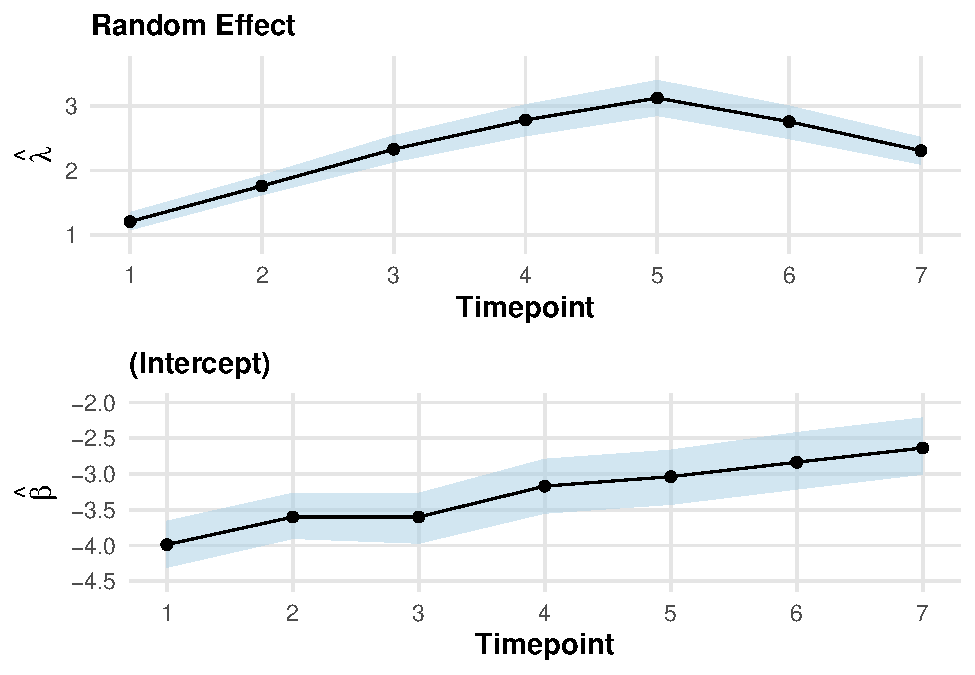
\includegraphics[width=0.7\linewidth]{Vignette-for-panelTVP_files/figure-latex/unnamed-chunk-34-1}

\begin{verbatim}
## The plots are out there, hit [Return] to see ...
\end{verbatim}

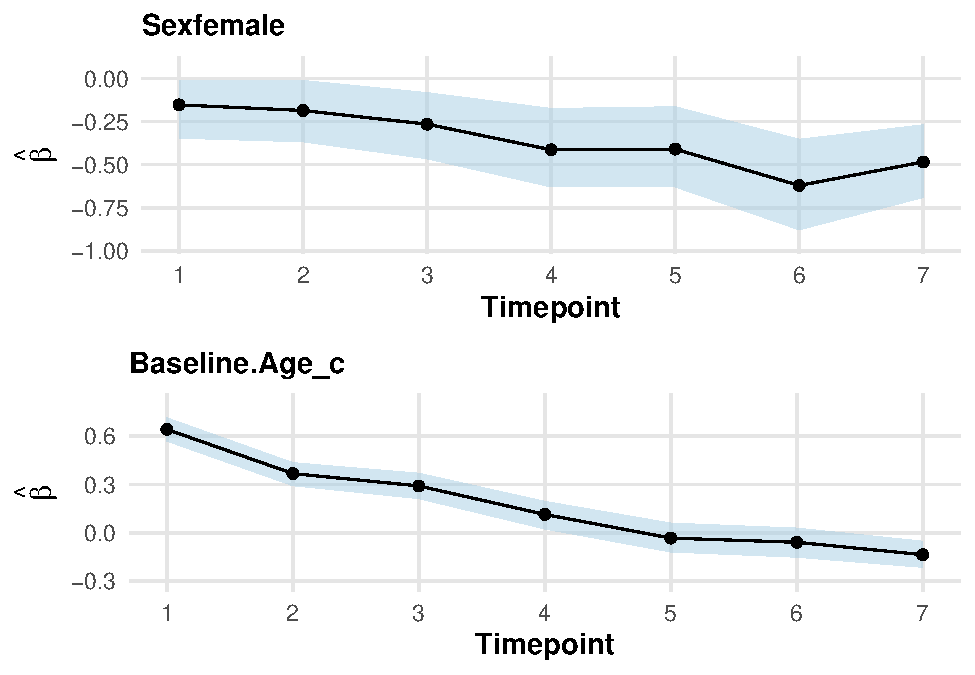
\includegraphics[width=0.7\linewidth]{Vignette-for-panelTVP_files/figure-latex/unnamed-chunk-34-2}

\begin{verbatim}
## The plots are out there, hit [Return] to see ...
\end{verbatim}

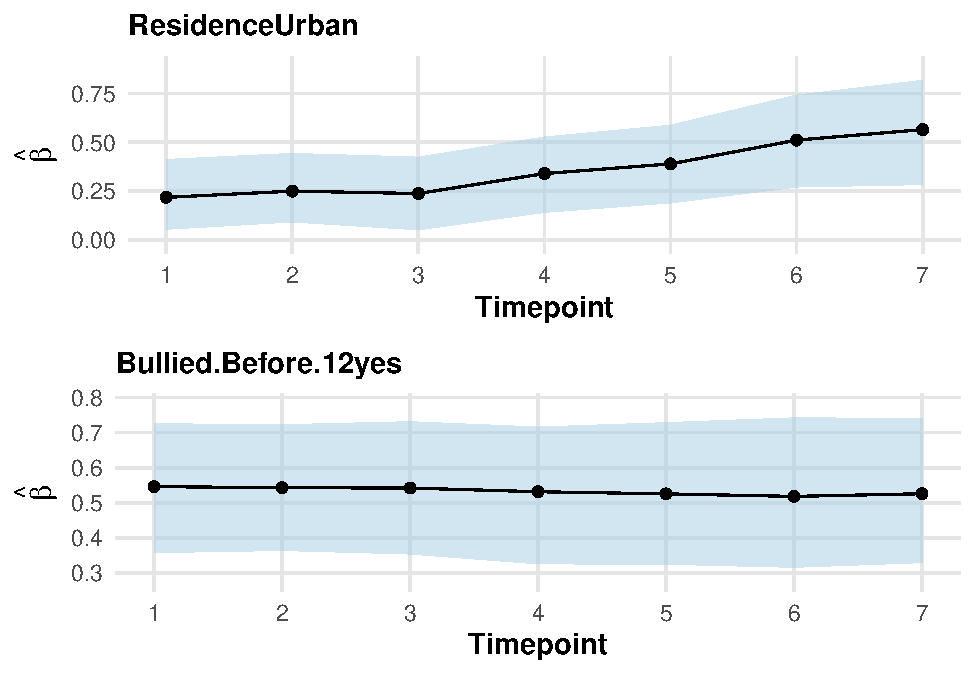
\includegraphics[width=0.7\linewidth]{Vignette-for-panelTVP_files/figure-latex/unnamed-chunk-34-3}

\begin{verbatim}
## The plots are out there, hit [Return] to see ...
\end{verbatim}

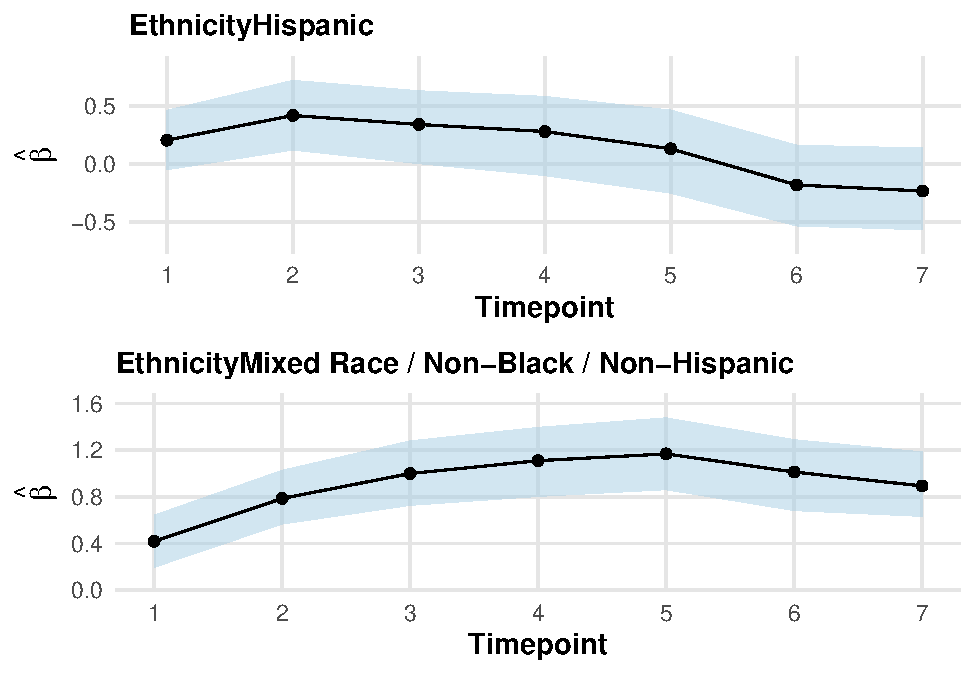
\includegraphics[width=0.7\linewidth]{Vignette-for-panelTVP_files/figure-latex/unnamed-chunk-34-4}

Based on the estimated effects, we see an increase in the probability of
Marijuana consumption over time - although the probability is, in
general, quite low. The effect of baseline age decreases almost linearly
over time and is close to zero in the second half of the study period.
People who live in urban areas are more likely to consume Marijuana than
those who live in rural areas. Moreover, this effect increases after the
third time point. If a person was bullied before the age of 12, he or
she has a higher probability of consuming Marijuana. This effect remains
constant over the study period. The person's ethnicity also influences
the consumption behavior and women are less likely to consume Marijuana
than men. Finally, the factor loading increases linearly until the fifth
panel wave and afterwards decreases linearly. Hence, the degree of
between-subject heterogeneity varies over time.

\section{Analyzing synthetic zero-inflated and overdispersed count
response
data}\label{analyzing-synthetic-zero-inflated-and-overdispersed-count-response-data}

In this section we describe how zero-inflated and overdispersed count
data can be analyzed with the \texttt{panelTVP()} function. We consider
synthetic data that we simulate using the function
\texttt{sim\_panelTVP()} and compare our shrinkage prior approach to an
unstructured approach, where independent Normal priors are placed on the
regression effects and the factor loadings.

The function \texttt{sim\_panelTVP()} has the following structure:

\begin{Shaded}
\begin{Highlighting}[]
\NormalTok{sim\_panelTVP(n, Tmax, model,}
\NormalTok{             beta = NULL, theta = NULL,}
\NormalTok{             lambda = NULL, psi = NULL,}
\NormalTok{             beta\_zinb.count = NULL, theta\_zinb.count = NULL,}
\NormalTok{             lambda\_zinb.count = NULL, psi\_zinb.count = NULL,}
\NormalTok{             beta\_zinb.inflation = NULL, theta\_zinb.inflation = NULL,}
\NormalTok{             lambda\_zinb.inflation = NULL, psi\_zinb.inflation = NULL, }
\NormalTok{             r = NULL, sigma2 = NULL)}
\end{Highlighting}
\end{Shaded}

Argument \texttt{n} is the number of subjects, whereas \texttt{Tmax} is
the total number of repeated measurements or time points. Both
parameters expect numeric scalars. The argument \texttt{model} defines
the model from which data are to be simulated. This argument expects one
of the following character strings \texttt{"Gaussian"},
\texttt{"Probit"}, \texttt{"Logit"}, \texttt{"NegBin"}, \texttt{"ZINB"}.
No aliases were given so the user is not allowed to deviate from these
naming conventions.

The regression effects and the factor loadings are then simulated from
the first-order random walks that were already discussed in the
theoretical chapter of this vignette. The parameter \texttt{beta} is the
vector of ``fixed effects'', whereas \texttt{theta} is the vector of
scale parameters for the random walks of the regression effects.
\texttt{lambda} and \texttt{psi} are both scalars and the starting value
as well as the scale parameter of the random walk for the factor
loading, respectively. As there are two linear predictors in the
Zero-Inflated Negative Binomial model, there are also two sets of random
walk parameters. The arguments ending at \texttt{inflation} are the
parameters for the Logit component, whereas the arguments ending at
\texttt{count} are the parameters for the Negative Binomial component.

Finally, the arguments \texttt{r} and \texttt{sigma2} refer to the
dispersion parameter of the Negative Binomial distribution and the
homoscedastic error variance of the Normal distribution, respectively.

In the following code chunck, data from a Zero-Inflated Negative
Binomial panel model are simulated and then analyzed with a random walk
shrinkage prior and an independence prior, respectively.

\bibliography{mybibfile.bib}


\end{document}
